% Options for packages loaded elsewhere
\PassOptionsToPackage{unicode}{hyperref}
\PassOptionsToPackage{hyphens}{url}
\PassOptionsToPackage{dvipsnames,svgnames,x11names}{xcolor}
%
\documentclass[
  letterpaper,
  DIV=11,
  numbers=noendperiod]{scrartcl}

\usepackage{amsmath,amssymb}
\usepackage{iftex}
\ifPDFTeX
  \usepackage[T1]{fontenc}
  \usepackage[utf8]{inputenc}
  \usepackage{textcomp} % provide euro and other symbols
\else % if luatex or xetex
  \usepackage{unicode-math}
  \defaultfontfeatures{Scale=MatchLowercase}
  \defaultfontfeatures[\rmfamily]{Ligatures=TeX,Scale=1}
\fi
\usepackage{lmodern}
\ifPDFTeX\else  
    % xetex/luatex font selection
\fi
% Use upquote if available, for straight quotes in verbatim environments
\IfFileExists{upquote.sty}{\usepackage{upquote}}{}
\IfFileExists{microtype.sty}{% use microtype if available
  \usepackage[]{microtype}
  \UseMicrotypeSet[protrusion]{basicmath} % disable protrusion for tt fonts
}{}
\makeatletter
\@ifundefined{KOMAClassName}{% if non-KOMA class
  \IfFileExists{parskip.sty}{%
    \usepackage{parskip}
  }{% else
    \setlength{\parindent}{0pt}
    \setlength{\parskip}{6pt plus 2pt minus 1pt}}
}{% if KOMA class
  \KOMAoptions{parskip=half}}
\makeatother
\usepackage{xcolor}
\setlength{\emergencystretch}{3em} % prevent overfull lines
\setcounter{secnumdepth}{-\maxdimen} % remove section numbering
% Make \paragraph and \subparagraph free-standing
\makeatletter
\ifx\paragraph\undefined\else
  \let\oldparagraph\paragraph
  \renewcommand{\paragraph}{
    \@ifstar
      \xxxParagraphStar
      \xxxParagraphNoStar
  }
  \newcommand{\xxxParagraphStar}[1]{\oldparagraph*{#1}\mbox{}}
  \newcommand{\xxxParagraphNoStar}[1]{\oldparagraph{#1}\mbox{}}
\fi
\ifx\subparagraph\undefined\else
  \let\oldsubparagraph\subparagraph
  \renewcommand{\subparagraph}{
    \@ifstar
      \xxxSubParagraphStar
      \xxxSubParagraphNoStar
  }
  \newcommand{\xxxSubParagraphStar}[1]{\oldsubparagraph*{#1}\mbox{}}
  \newcommand{\xxxSubParagraphNoStar}[1]{\oldsubparagraph{#1}\mbox{}}
\fi
\makeatother

\usepackage{color}
\usepackage{fancyvrb}
\newcommand{\VerbBar}{|}
\newcommand{\VERB}{\Verb[commandchars=\\\{\}]}
\DefineVerbatimEnvironment{Highlighting}{Verbatim}{commandchars=\\\{\}}
% Add ',fontsize=\small' for more characters per line
\usepackage{framed}
\definecolor{shadecolor}{RGB}{241,243,245}
\newenvironment{Shaded}{\begin{snugshade}}{\end{snugshade}}
\newcommand{\AlertTok}[1]{\textcolor[rgb]{0.68,0.00,0.00}{#1}}
\newcommand{\AnnotationTok}[1]{\textcolor[rgb]{0.37,0.37,0.37}{#1}}
\newcommand{\AttributeTok}[1]{\textcolor[rgb]{0.40,0.45,0.13}{#1}}
\newcommand{\BaseNTok}[1]{\textcolor[rgb]{0.68,0.00,0.00}{#1}}
\newcommand{\BuiltInTok}[1]{\textcolor[rgb]{0.00,0.23,0.31}{#1}}
\newcommand{\CharTok}[1]{\textcolor[rgb]{0.13,0.47,0.30}{#1}}
\newcommand{\CommentTok}[1]{\textcolor[rgb]{0.37,0.37,0.37}{#1}}
\newcommand{\CommentVarTok}[1]{\textcolor[rgb]{0.37,0.37,0.37}{\textit{#1}}}
\newcommand{\ConstantTok}[1]{\textcolor[rgb]{0.56,0.35,0.01}{#1}}
\newcommand{\ControlFlowTok}[1]{\textcolor[rgb]{0.00,0.23,0.31}{\textbf{#1}}}
\newcommand{\DataTypeTok}[1]{\textcolor[rgb]{0.68,0.00,0.00}{#1}}
\newcommand{\DecValTok}[1]{\textcolor[rgb]{0.68,0.00,0.00}{#1}}
\newcommand{\DocumentationTok}[1]{\textcolor[rgb]{0.37,0.37,0.37}{\textit{#1}}}
\newcommand{\ErrorTok}[1]{\textcolor[rgb]{0.68,0.00,0.00}{#1}}
\newcommand{\ExtensionTok}[1]{\textcolor[rgb]{0.00,0.23,0.31}{#1}}
\newcommand{\FloatTok}[1]{\textcolor[rgb]{0.68,0.00,0.00}{#1}}
\newcommand{\FunctionTok}[1]{\textcolor[rgb]{0.28,0.35,0.67}{#1}}
\newcommand{\ImportTok}[1]{\textcolor[rgb]{0.00,0.46,0.62}{#1}}
\newcommand{\InformationTok}[1]{\textcolor[rgb]{0.37,0.37,0.37}{#1}}
\newcommand{\KeywordTok}[1]{\textcolor[rgb]{0.00,0.23,0.31}{\textbf{#1}}}
\newcommand{\NormalTok}[1]{\textcolor[rgb]{0.00,0.23,0.31}{#1}}
\newcommand{\OperatorTok}[1]{\textcolor[rgb]{0.37,0.37,0.37}{#1}}
\newcommand{\OtherTok}[1]{\textcolor[rgb]{0.00,0.23,0.31}{#1}}
\newcommand{\PreprocessorTok}[1]{\textcolor[rgb]{0.68,0.00,0.00}{#1}}
\newcommand{\RegionMarkerTok}[1]{\textcolor[rgb]{0.00,0.23,0.31}{#1}}
\newcommand{\SpecialCharTok}[1]{\textcolor[rgb]{0.37,0.37,0.37}{#1}}
\newcommand{\SpecialStringTok}[1]{\textcolor[rgb]{0.13,0.47,0.30}{#1}}
\newcommand{\StringTok}[1]{\textcolor[rgb]{0.13,0.47,0.30}{#1}}
\newcommand{\VariableTok}[1]{\textcolor[rgb]{0.07,0.07,0.07}{#1}}
\newcommand{\VerbatimStringTok}[1]{\textcolor[rgb]{0.13,0.47,0.30}{#1}}
\newcommand{\WarningTok}[1]{\textcolor[rgb]{0.37,0.37,0.37}{\textit{#1}}}

\providecommand{\tightlist}{%
  \setlength{\itemsep}{0pt}\setlength{\parskip}{0pt}}\usepackage{longtable,booktabs,array}
\usepackage{calc} % for calculating minipage widths
% Correct order of tables after \paragraph or \subparagraph
\usepackage{etoolbox}
\makeatletter
\patchcmd\longtable{\par}{\if@noskipsec\mbox{}\fi\par}{}{}
\makeatother
% Allow footnotes in longtable head/foot
\IfFileExists{footnotehyper.sty}{\usepackage{footnotehyper}}{\usepackage{footnote}}
\makesavenoteenv{longtable}
\usepackage{graphicx}
\makeatletter
\def\maxwidth{\ifdim\Gin@nat@width>\linewidth\linewidth\else\Gin@nat@width\fi}
\def\maxheight{\ifdim\Gin@nat@height>\textheight\textheight\else\Gin@nat@height\fi}
\makeatother
% Scale images if necessary, so that they will not overflow the page
% margins by default, and it is still possible to overwrite the defaults
% using explicit options in \includegraphics[width, height, ...]{}
\setkeys{Gin}{width=\maxwidth,height=\maxheight,keepaspectratio}
% Set default figure placement to htbp
\makeatletter
\def\fps@figure{htbp}
\makeatother

\KOMAoption{captions}{tableheading}
\makeatletter
\@ifpackageloaded{caption}{}{\usepackage{caption}}
\AtBeginDocument{%
\ifdefined\contentsname
  \renewcommand*\contentsname{Table of contents}
\else
  \newcommand\contentsname{Table of contents}
\fi
\ifdefined\listfigurename
  \renewcommand*\listfigurename{List of Figures}
\else
  \newcommand\listfigurename{List of Figures}
\fi
\ifdefined\listtablename
  \renewcommand*\listtablename{List of Tables}
\else
  \newcommand\listtablename{List of Tables}
\fi
\ifdefined\figurename
  \renewcommand*\figurename{Figure}
\else
  \newcommand\figurename{Figure}
\fi
\ifdefined\tablename
  \renewcommand*\tablename{Table}
\else
  \newcommand\tablename{Table}
\fi
}
\@ifpackageloaded{float}{}{\usepackage{float}}
\floatstyle{ruled}
\@ifundefined{c@chapter}{\newfloat{codelisting}{h}{lop}}{\newfloat{codelisting}{h}{lop}[chapter]}
\floatname{codelisting}{Listing}
\newcommand*\listoflistings{\listof{codelisting}{List of Listings}}
\makeatother
\makeatletter
\makeatother
\makeatletter
\@ifpackageloaded{caption}{}{\usepackage{caption}}
\@ifpackageloaded{subcaption}{}{\usepackage{subcaption}}
\makeatother
\makeatletter
\@ifpackageloaded{fontawesome5}{}{\usepackage{fontawesome5}}
\makeatother
\ifLuaTeX
  \usepackage{selnolig}  % disable illegal ligatures
\fi
\usepackage{bookmark}

\IfFileExists{xurl.sty}{\usepackage{xurl}}{} % add URL line breaks if available
\urlstyle{same} % disable monospaced font for URLs
\hypersetup{
  pdftitle={Reproducible Manuscripts},
  pdfauthor={Alexander Mark Weber},
  colorlinks=true,
  linkcolor={blue},
  filecolor={Maroon},
  citecolor={Blue},
  urlcolor={Blue},
  pdfcreator={LaTeX via pandoc}}

\title{Reproducible Manuscripts}
\author{Alexander Mark Weber}
\date{2024-06-26}

\begin{document}
\maketitle

\subsection{Notes}\label{notes}

\section{Bridge-In}\label{bridge-in}

\subsection{Mentimeter}\label{mentimeter}

\subsection{Scientific Method}\label{scientific-method}

\subsection{Scientific Method}\label{scientific-method-1}

What is the scientific method (broadly)?

\begin{enumerate}
\def\labelenumi{\arabic{enumi}.}
\item
  Define a question
\item
  Gather information and resources (observe)
\item
  Form an explanatory hypothesis
\item
  Test the hypothesis by performing an experiment and collecting data in
  a reproducible manner
\item
  Analyze the data
\item
  Interpret the data and draw conclusions that serve as a starting point
  for a new hypothesis
\item
  Publish results
\item
  Retest (frequently done by other scientists)
\end{enumerate}

\subsection{Scientific Method}\label{scientific-method-2}

\begin{enumerate}
\def\labelenumi{\arabic{enumi}.}
\setcounter{enumi}{6}
\tightlist
\item
  Publish Results
\item
  Retest (frequently done by other scientists)
\end{enumerate}

\subsection{Problem}\label{problem}

\begin{itemize}
\tightlist
\item
  In 2011, John Ioannidis\footnote{Ioannidis JPA (2005) Why most
    published research findings are false. PLoS Med 2(8): e124.}
  published 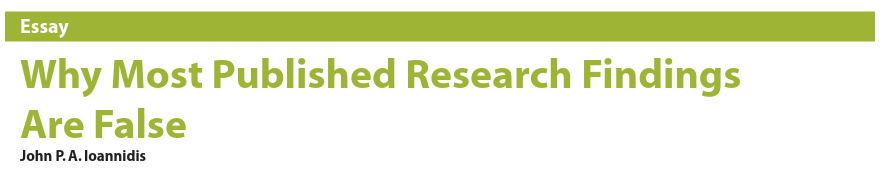
\includegraphics{img/IoannidisPaper.png}
\item
  Why?

  \begin{itemize}
  \tightlist
  \item
    Studies are underpowered
  \item
    Current incentives lead scientists to publish quantity over quality
  \item
    No incentives for scientists to replicate other studies
  \item
    More\ldots{}
  \end{itemize}
\end{itemize}

John suggested that the majority of all published papers at the time
were likely not true. Or put another way, wouldn't be reproduced

\subsection{Problem}\label{problem-1}

Was he right?

\begin{itemize}
\tightlist
\item
  In 2015, the Open Science Collaboration sampled studies from prominent
  journals to estimate the replicability of psychological
  research.\footnote{Open Science Collaboration. Estimating the
    reproducibility of psychological science. Science 349, aac4716
    (2015).}
\end{itemize}

\subsection{Problem}\label{problem-2}

\subsection{Problem}\label{problem-3}

\begin{Shaded}
\begin{Highlighting}[]
\CommentTok{\# Load ggplot2}
\FunctionTok{library}\NormalTok{(ggplot2)}
\FunctionTok{library}\NormalTok{(tidyverse)}
\end{Highlighting}
\end{Shaded}

\begin{verbatim}
-- Attaching packages --------------------------------------- tidyverse 1.3.1 --
\end{verbatim}

\begin{verbatim}
v tibble  3.2.1     v dplyr   1.1.4
v tidyr   1.3.1     v stringr 1.5.1
v readr   2.1.5     v forcats 0.5.1
v purrr   1.0.2     
\end{verbatim}

\begin{verbatim}
-- Conflicts ------------------------------------------ tidyverse_conflicts() --
x dplyr::filter() masks stats::filter()
x dplyr::lag()    masks stats::lag()
\end{verbatim}

\begin{Shaded}
\begin{Highlighting}[]
\CommentTok{\# Create Data}
\NormalTok{data }\OtherTok{\textless{}{-}} \FunctionTok{data.frame}\NormalTok{(}
  \AttributeTok{group=}\FunctionTok{c}\NormalTok{(}\StringTok{"Successful"}\NormalTok{, }\StringTok{"Unsuccessful"}\NormalTok{),}
  \AttributeTok{value=}\FunctionTok{c}\NormalTok{(}\DecValTok{39}\NormalTok{,}\DecValTok{61}\NormalTok{)}
\NormalTok{)}

\NormalTok{data }\OtherTok{\textless{}{-}}\NormalTok{ data }\SpecialCharTok{|\textgreater{}}
  \FunctionTok{arrange}\NormalTok{(}\FunctionTok{desc}\NormalTok{(group)) }\SpecialCharTok{|\textgreater{}}
  \FunctionTok{mutate}\NormalTok{(}\AttributeTok{prop =}\NormalTok{ value }\SpecialCharTok{/} \FunctionTok{sum}\NormalTok{(data}\SpecialCharTok{$}\NormalTok{value) }\SpecialCharTok{*}\DecValTok{100}\NormalTok{) }\SpecialCharTok{|\textgreater{}}
  \FunctionTok{mutate}\NormalTok{(}\AttributeTok{ypos =} \FunctionTok{cumsum}\NormalTok{(prop)}\SpecialCharTok{{-}} \FloatTok{0.5}\SpecialCharTok{*}\NormalTok{prop )}

\CommentTok{\# Basic piechart}
\FunctionTok{ggplot}\NormalTok{(data, }\FunctionTok{aes}\NormalTok{(}\AttributeTok{x=}\StringTok{""}\NormalTok{, }\AttributeTok{y=}\NormalTok{value, }\AttributeTok{fill=}\NormalTok{group)) }\SpecialCharTok{+}
  \FunctionTok{geom\_bar}\NormalTok{(}\AttributeTok{stat=}\StringTok{"identity"}\NormalTok{, }\AttributeTok{width=}\DecValTok{1}\NormalTok{, }\AttributeTok{color=}\StringTok{"white"}\NormalTok{) }\SpecialCharTok{+}
  \FunctionTok{coord\_polar}\NormalTok{(}\StringTok{"y"}\NormalTok{, }\AttributeTok{start=}\DecValTok{0}\NormalTok{) }\SpecialCharTok{+} \FunctionTok{theme\_void}\NormalTok{() }\SpecialCharTok{+}
  \FunctionTok{theme}\NormalTok{(}\AttributeTok{legend.text =} \FunctionTok{element\_text}\NormalTok{(}\AttributeTok{size=}\DecValTok{18}\NormalTok{), }\AttributeTok{legend.title =} \FunctionTok{element\_blank}\NormalTok{())}\SpecialCharTok{+}

  \FunctionTok{geom\_text}\NormalTok{(}\FunctionTok{aes}\NormalTok{(}\AttributeTok{y =}\NormalTok{ ypos, }\AttributeTok{label =}\NormalTok{ value), }\AttributeTok{color =} \StringTok{"white"}\NormalTok{, }\AttributeTok{size=}\DecValTok{6}\NormalTok{) }\SpecialCharTok{+}
  \FunctionTok{scale\_fill\_brewer}\NormalTok{(}\AttributeTok{palette=}\StringTok{"Set1"}\NormalTok{)}
\end{Highlighting}
\end{Shaded}

\begin{figure}[H]

\centering{

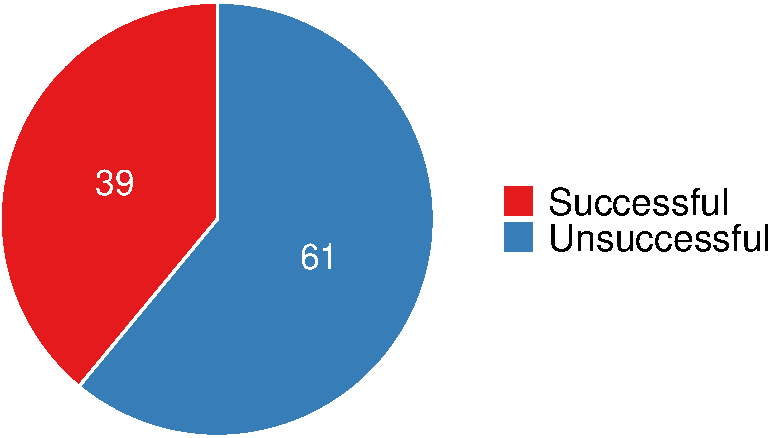
\includegraphics{ReproducibleManuscript_files/figure-pdf/fig-opensci-1.pdf}

}

\caption{\label{fig-opensci}}

\end{figure}%

Out of 100 independently performed replications, only 39\% were
subjectively labelled as successful replications, and on average, the
effects were roughly half the original size \footnote{https://www.nature.com/articles/s44271-023-00003-2}

{[}https://www.nature.com/articles/s44271-023-00003-2{]}

Out of 100 independently performed replications, only 39\% were
subjectively labelled as successful replications, and on average, the
effects were roughly half the original size

\subsection{Problem}\label{problem-4}

Not just in Psychology:

\begin{itemize}
\tightlist
\item
  animal behaviour\footnote{Farrar, B. G., Boeckle, M. \& Clayton, N. S.
    Replications in comparative cognition: what should we expect and how
    can we improve? Anim. Behav. Cognit. 7, 1 (2020).};
\item
  cancer biology\footnote{Errington, T. M. et al.~Investigating the
    replicability of preclinical cancer biology. Elife 10, e71601
    (2021).};
\item
  economics\footnote{Camerer, C. F. et al.~Evaluating replicability of
    laboratory experiments in economics. Science 351, 1433--1436 (2016).}
\item
  pharmaceutical industry\footnote{Begley CG, Ellis LM (2012) Drug
    development: Raise standards for preclinical cancer research. Nature
    483: 531--533. doi: 10.1038/483531a PMID: 22460880}
\item
  neuroscience\footnote{K.S. Button, J.P.A. Ioannidis, C. Mokrysz, B.A.
    Nosek, J. Flint, E.S.J. Robinson, M.R. Munafò. Power failure: Why
    small sample size undermines the reliability of neuroscience. Nat
    Rev Neurosci, 14 (2013), pp.~365-376}
\item
  neuroimaging\footnote{Marek, S., Tervo-Clemmens, B., Calabro, F.J. et
    al.~Reproducible brain-wide association studies require thousands of
    individuals. Nature 603, 654--660 (2022).
    https://doi.org/10.1038/s41586-022-04492-9}
\item
  clinical trials\footnote{Carlisle, J. B. Anaesthesia 76, 472--479
    (2021).}
\end{itemize}

\subsection{Problem}\label{problem-5}

\begin{itemize}
\tightlist
\item
  For clinical trials: 44\% contained at least some flawed
  data:\footnote{Carlisle, J. B. Anaesthesia 76, 472--479 (2021).}

  \begin{itemize}
  \tightlist
  \item
    impossible statistics,
  \item
    incorrect calculations,
  \item
    or duplicated numbers or figures
  \item
    26\% of trials were impossible to judge: either due to incompetence
    or faked data
  \end{itemize}
\end{itemize}

\subsection{Problem}\label{problem-6}

\begin{itemize}
\item
  Publishing irreproducible results is worse than not publishing: more
  difficult to eliminate an idea than it is to introduce it\footnote{C.
    Piller. Disgraced COVID-19 studies are still routinely cited.
    Science, 371 (2021), pp.~331-332; E.M. Bucci. On zombie papers. Cell
    Death Dis, 10 (2019), p.~189; S.B. Nissen, T. Magidson, K. Gross,
    C.T. Bergstrom. Publication bias and the canonization of false
    facts. eLife, 5 (2016), Article e21451}
\item
  Spurious results can mislead other researchers who conduct follow-up
  investigations or try to integrate findings into broader theories.
\end{itemize}

For the clinical trials; for more than 150 trials, the author of the
paper got access to anonymized individual participant data (IPD). By
studying the IPD spreadsheets, he judged that 44\% of these trials
contained at least some flawed data: impossible statistics, incorrect
calculations or duplicated numbers or figures, for instance. And 26\% of
the papers had problems that were so widespread that the trial was
impossible to trust, he judged --- either because the authors were
incompetent, or because they had faked the data.

\subsection{What Can We Do?}\label{what-can-we-do}

\begin{itemize}
\item
  Many solutions are needed; far outside the scope of this talk
\item
  \textbf{One thing we can do is change the way we write papers.}
  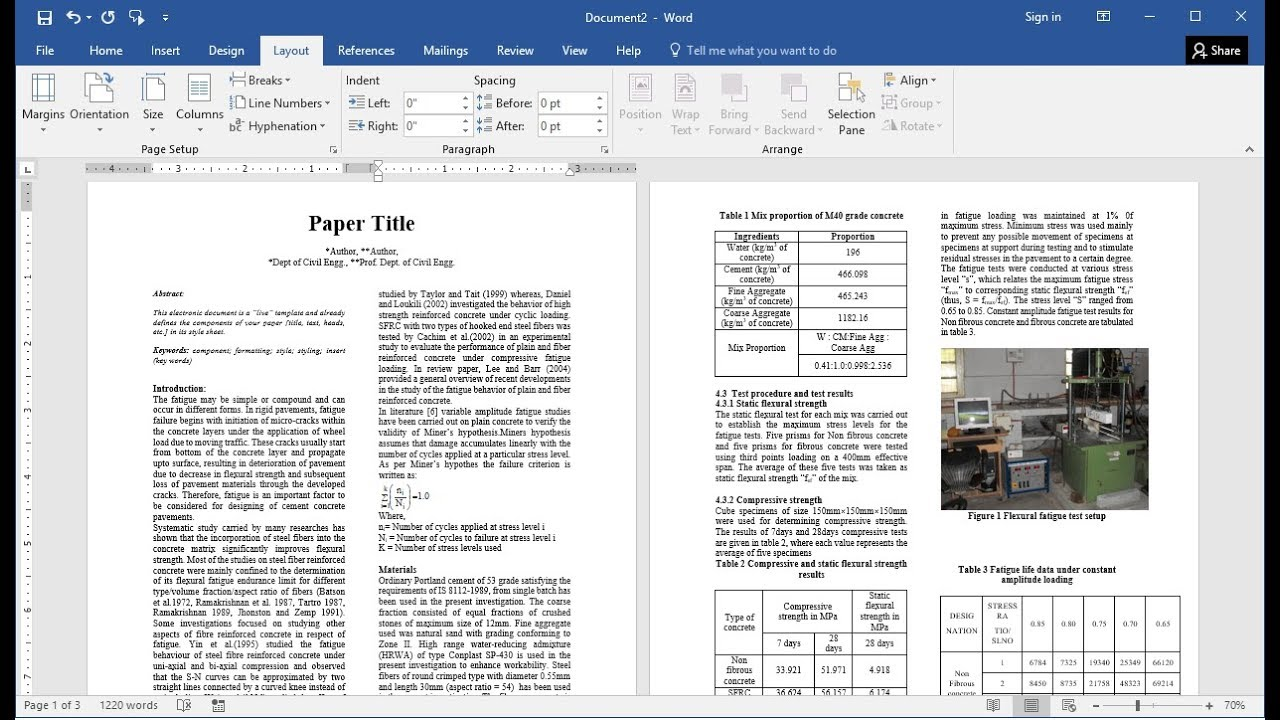
\includegraphics[width=0.55\textwidth,height=0.55\textheight]{img/worddoc.png}
\item
  Currently, papers are written and published in a way that results in
  \textbf{errors} and the inability to \textbf{computationally
  reproduce} results.
\end{itemize}

\subsection{What Can We Do?}\label{what-can-we-do-1}

\begin{itemize}
\tightlist
\item
  \textbf{Errors}: a 2016 paper by Nuijten et al.\footnote{Nuijten,
    Michèle B, Chris HJ Hartgerink, Marcel ALM van Assen, Sacha Epskamp,
    and Jelte M Wicherts. 2016. ``The Prevalence of Statistical
    Reporting Errors in Psychology (1985--2013).'' Behavior Research
    Methods 48 (4). Springer: 1205--26.} found that

  \begin{itemize}
  \tightlist
  \item
    nearly \textbf{half} of all papers had errors in them;
  \item
    over \textbf{10\%} of p-values in published papers were inconsistent
    with the reported details of the statistical test
  \item
    1.6\% were what they called ``grossly'' inconsistent,
    e.g.~difference between the p-value and the test statistic meant
    that one implied statistical significance and the other did not
  \end{itemize}
\end{itemize}

\subsection{What Can We Do?}\label{what-can-we-do-2}

\begin{itemize}
\tightlist
\item
  \textbf{Computational reproducibility}: a 2021 paper by Hardwicke et
  al.\footnote{T.E. Hardwicke, M. Bohn, K. MacDonald, E. Hembacher, M.B.
    Nuijten, B.N. Peloquin, et al.~Analytic reproducibility in articles
    receiving open data badges at the journal Psychological Science: An
    observational study. R Soc Open Sci, 8 (2021), Article 201494}
  attempted to reproduce results from 25 published papers that publicly
  shared their data and code:

  \begin{itemize}
  \tightlist
  \item
    found substantial numerical discrepancies between reported
    statistical values and values obtained from reproduction attempts in
    \textbf{64\%} of these papers
  \end{itemize}
\end{itemize}

\subsection{What Can We Do?}\label{what-can-we-do-3}

This is where \textbf{Reproducible Papers} come in\ldots{}

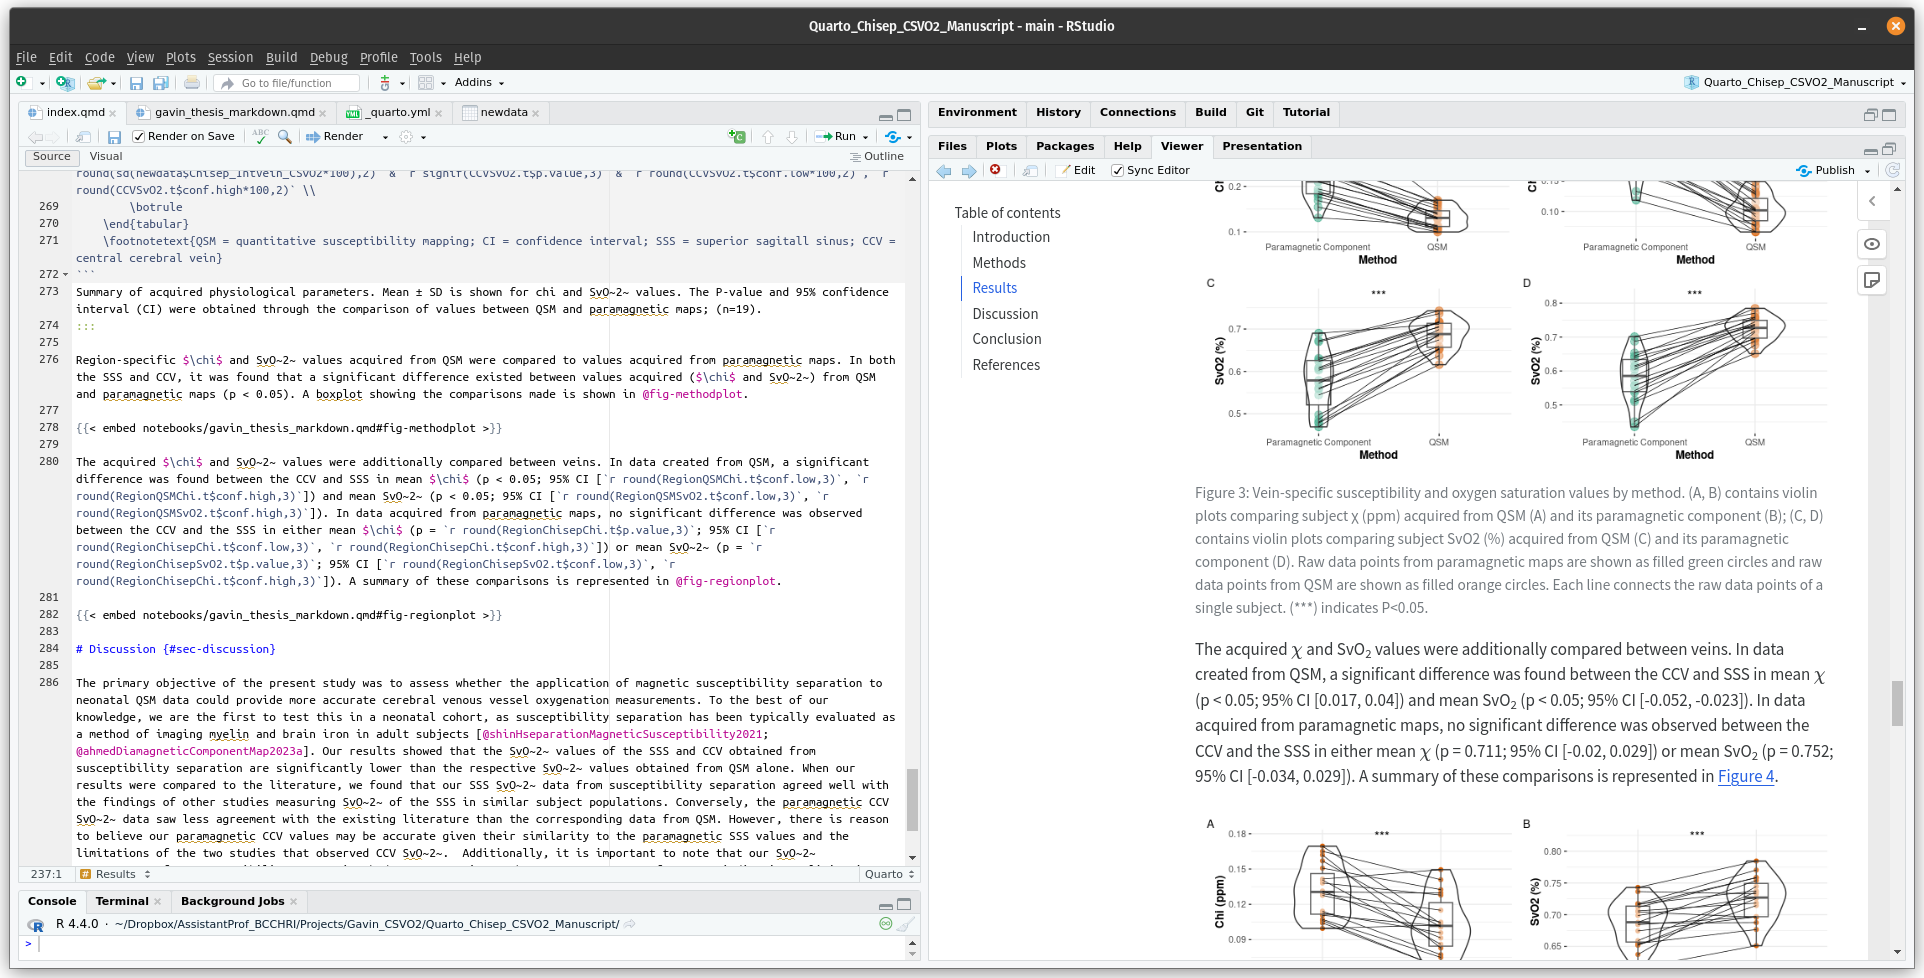
\includegraphics{img/reprocpaper_example.png}

\section{Learning Goals}\label{learning-goals}

\subsection{Learning Goals}\label{learning-goals-1}

By the end of the talk, the audience should:

\begin{itemize}
\tightlist
\item
  Know what a reproducible manuscript is,
\item
  Understand some reasons why scientists should be writing their
  manuscripts this way,
\item
  Know what Markdown, Knitr, Pandoc, LaTeX, Jupyter Notebook,
  R/RMarkdown, and Quarto are,
\item
  Know the basics of the syntax for Markdown, R and Quarto,
\item
  See how to integrate author information, code, equations, tables,
  images, and citations
\item
  Be able to start writing your next manuscript using Quarto Manuscripts
\end{itemize}

\section{Introduction}\label{introduction}

\subsection{What is a reproducible
manuscript?}\label{what-is-a-reproducible-manuscript}

\begin{itemize}
\tightlist
\item
  Reports the scientific findings
\item
  Provides all (or almost all) the necessary data, code, and
  methodologies required to create those findings (i.e.~data, stats,
  figures, tables, etc.)
\item
  Transparent and organized
\item
  Enables others to \textbf{replicate} and \textbf{verify} the results
  of your study independently
\end{itemize}


\includegraphics{img/qmark.png}

\subsection{What does it look like?}\label{what-does-it-look-like}

\begin{Shaded}
\begin{Highlighting}[]
\NormalTok{{-}{-}{-}}
\NormalTok{title: "The Application of Magnetic Susceptibility Separation for Measuring Cerebral Oxygenation in Preterm Neonates"}
\NormalTok{titlerunning: "CSVO2"}
\NormalTok{author:}
\NormalTok{  {-} name: Thomas Gavin Carmichael}
\NormalTok{    orcid: 0009{-}0008{-}6849{-}5333}
\NormalTok{    corresponding: false}
\NormalTok{    email: tgcarmichael@outlook.com}
\NormalTok{    roles:}
\NormalTok{      {-} writing {-} original draft}
\NormalTok{      {-} formal analysis}
\NormalTok{      {-} methodology}
\NormalTok{      {-} validation}
\NormalTok{      {-} visualization}
\NormalTok{    affiliations:}
\NormalTok{      {-} ref: 1}
\NormalTok{      {-} ref: 2}
\NormalTok{    degrees:}
\NormalTok{      {-} HBSc}
\NormalTok{  {-} name: Alexander Rauscher}
\NormalTok{    orcid: 0000{-}0002{-}1961{-}8252}
\NormalTok{    email: rauscher@physics.ubc.ca}
\NormalTok{    corresponding: false}
\NormalTok{    roles:}
\NormalTok{      {-} writing {-} review \& editing}
\NormalTok{    affiliations:}
\NormalTok{      {-} ref: 3}
\NormalTok{    degrees:}
\NormalTok{      {-} PhD}
\NormalTok{      {-} MSc}
\NormalTok{  {-} name: Ruth E Grunau}
\NormalTok{    orcid: 0000{-}0002{-}5428{-}9212}
\NormalTok{    corresponding: false}
\NormalTok{    email: rgrunau@mail.ubc.ca}
\NormalTok{    roles:}
\NormalTok{      {-} writing {-} review \& editing}
\NormalTok{      {-} funding acquisition}
\NormalTok{    affiliations:}
\NormalTok{      {-} ref: 2}
\NormalTok{      {-} ref: 3}
\NormalTok{  {-} name: Alexander Mark Weber}
\NormalTok{    orcid: 0000{-}0001{-}7295{-}0775}
\NormalTok{    corresponding: true}
\NormalTok{    email: aweber@bcchr.ca}
\NormalTok{    roles:}
\NormalTok{      {-} project administration}
\NormalTok{      {-} supervision}
\NormalTok{      {-} validation}
\NormalTok{      {-} visualization}
\NormalTok{      {-} resources}
\NormalTok{      {-} methodology}
\NormalTok{      {-} formal analysis}
\NormalTok{      {-} funding acquisition}
\NormalTok{      {-} writing {-} review \& editing}
\NormalTok{      {-} conceptualization}
\NormalTok{      {-} data curation}
\NormalTok{      {-} investigation}
\NormalTok{    affiliations:}
\NormalTok{      {-} ref: 2}
\NormalTok{      {-} ref: 3}
\NormalTok{    degrees:}
\NormalTok{      {-} PhD}
\NormalTok{      {-} MSc}
\NormalTok{affiliations:}
\NormalTok{  {-} id: 1}
\NormalTok{    name: The University of British Columbia}
\NormalTok{    department: Integrated Sciences}
\NormalTok{    address: 2329 West Mall}
\NormalTok{    city: Vancouver}
\NormalTok{    region: BC}
\NormalTok{    country: Canada}
\NormalTok{    postal{-}code: V6T 1Z4}
\NormalTok{  {-} id: 3}
\NormalTok{    name: The University of British Columbia}
\NormalTok{    department: Pediatrics}
\NormalTok{    address: 2329 West Mall}
\NormalTok{    city: Vancouver}
\NormalTok{    region: BC}
\NormalTok{    country: Canada}
\NormalTok{    postal{-}code: V6T 1Z4}
\NormalTok{  {-} id: 2}
\NormalTok{    department: BC Children\textquotesingle{}s Hospital Research Institute}
\NormalTok{    name: The University of British Columbia}
\NormalTok{    address: 938 West 28th Avenue}
\NormalTok{    city: Vancouver}
\NormalTok{    state: BC}
\NormalTok{    country: Canada}
\NormalTok{    postal{-}code: V5Z 4H4}

\NormalTok{keywords:}
\NormalTok{  {-} Quantitative Susceptbility Mapping}
\NormalTok{  {-} Preterm}
\NormalTok{  {-} Newborn}
\NormalTok{  {-} Cerebral Venous Oxygen Saturation}
\NormalTok{abstract: |}
\NormalTok{  **Background**: Quantitative susceptibility mapping (QSM) is a magnetic resonance imaging (MRI) modality proposed to be a viable method of measuring cerebral oxygenation in neonates given its sensitivity to deoxyhemoglobin, a paramagnetic molecule. During QSM, however, paramagnetic sources can be obscured by opposing diamagnetic sources such as water and myelin. We sought to evaluate whether QSM images alone, or an algorithm that attempts to isolate their paramagnetic components, are more accurate in measuring oxygenation of the major cerebral veins in a cohort of neonates born preterm. Additionally, we aimed to determine whether a difference in oxygenation existed between the major cerebral veins.}
  
\NormalTok{  **Methods**: 19 neonates born preterm were scanned on a 3T research MRI at term equivalent age. The protocol included a multi{-}echo susceptibility{-}weighted imaging sequence. The acquired imaging data were processed as QSM images to obtain the susceptibility values of the superior sagittal sinus (SSS) and central cerebral veins (CCV). These values were used to calculate the oxygen saturation (SvO\textasciitilde{}2\textasciitilde{}) of the SSS and CCV.  QSM images were subsequently processed to isolate their paramagnetic components. SvO\textasciitilde{}2\textasciitilde{} values of the SSS and CCV were calculated again from the paramagnetic components.}
  
\NormalTok{  **Results**: The mean SvO\textasciitilde{}2\textasciitilde{} values of the SSS and CCV calculated from QSM images were found to be 72.4\% (SD, 3.4\%) and 68.7\% (SD, 3.5\%), respectively. The mean SvO\textasciitilde{}2\textasciitilde{} values calculated from paramagnetic components were found to be 58.1\% (SD, 7.3\%) for the SSS and 57.7\% (SD, 7.0\%) for the CCV.}
  
\NormalTok{  **Conclusion**: SSS SvO\textasciitilde{}2\textasciitilde{} values derived from paramagnetic components agreed well with the existing literature and were closer than the values derived from QSM, however, they displayed greater variability. Although the CCV SvO\textasciitilde{}2\textasciitilde{} data from QSM aligns more closely with existing literature, it is important to note that the current literature on this topic remains relatively limited in the CCV. Thus, decomposing QSM images into paramagnetic components shows great promise as a method for more accurately measuring cerebral oxygenation in neonates but may require more research to improve precision. Notably, no significant difference in oxygenation was observed between the CCV and the SSS, contrasting with previous studies.}
  
\NormalTok{plain{-}language{-}summary: |}
  
\NormalTok{key{-}points:}
\NormalTok{  {-} }
\NormalTok{date: last{-}modified}
\NormalTok{bibliography: [ Gavin\_Thesis\_Ref.bib ]}
\NormalTok{citation:}
\NormalTok{  container{-}title: Unpublished}
\NormalTok{number{-}sections: false}
\NormalTok{notebook{-}links: true}
\NormalTok{{-}{-}{-}}

\NormalTok{\textasciigrave{}\textasciigrave{}\textasciigrave{}\{r setup, include=FALSE\}}
\NormalTok{\# options}
\NormalTok{knitr::opts\_chunk$set(}
\NormalTok{  \# fig.width=8, fig.height=5, }
\NormalTok{  \# out.width="50\%",}
\NormalTok{  \# fig.align="center",}
\NormalTok{  echo=FALSE, }
\NormalTok{  message=FALSE, }
\NormalTok{  warning=FALSE}
\NormalTok{  \# cache=TRUE }
\NormalTok{  )}
\NormalTok{set.seed(1234) \# reproducible}
\NormalTok{options(knitr.kable.NA = \textquotesingle{}\textquotesingle{}) \# how kable handles NA}
\NormalTok{options(reticulate.repl.quiet = TRUE)}
\NormalTok{\textasciigrave{}\textasciigrave{}\textasciigrave{}}

\NormalTok{\textasciigrave{}\textasciigrave{}\textasciigrave{}\{r libraries\}}
\NormalTok{\#libraries}
\NormalTok{library(tidyverse) \# ggplot2, dplyr, tidyr, readr, purrr, tibble, stringr, forcats}
\NormalTok{theme\_set( theme\_minimal() ) \# ggplot theme}
\NormalTok{library(broom) \# for nice summaries}
\NormalTok{library(knitr) \# }
\NormalTok{library(kableExtra) \# more tables options. Can cause problems}
\NormalTok{library(Rmpfr)}
\NormalTok{library(gt)}
\NormalTok{\# library(reticulate) \# incorporate Python}
\NormalTok{\# use\_virtualenv(\textquotesingle{}./pyvenv\_csvo\textquotesingle{}, required = TRUE) \# load pythong venv from path}

\NormalTok{\# library(neurobase)}
\NormalTok{\textasciigrave{}\textasciigrave{}\textasciigrave{}}

\NormalTok{\textasciigrave{}\textasciigrave{}\textasciigrave{}\{r\}}
\NormalTok{load("notebooks/results.RData")}
\NormalTok{\textasciigrave{}\textasciigrave{}\textasciigrave{}}

\NormalTok{\textasciigrave{}\textasciigrave{}\textasciigrave{}\{r\}}
\NormalTok{\# function to make rounding means and sd easier}
\NormalTok{rndmean \textless{}{-} function(clm) \{}
\NormalTok{  return(round(mean(clm),2))}
\NormalTok{\}}
\NormalTok{rndsd \textless{}{-} function(clm) \{}
\NormalTok{  return(round(sd(clm),2))}
\NormalTok{\}}
\NormalTok{\textasciigrave{}\textasciigrave{}\textasciigrave{}}

\NormalTok{\# Introduction \{\#sec{-}intro\}}

\NormalTok{\textless{}!{-}{-} should be around 5{-}6 paragraphs. Aim for 460 words {-}{-}\textgreater{}}

\NormalTok{Preterm birth }

\NormalTok{Abnormal brain development is a significant concern for parents with children born preterm, as 43\% of infants that survive will have neurodevelopmental delays later in life [@dixMonitoringCerebralOxygenation2017]. Irregularities in early cerebral oxygen levels have been identified as a potential source of such delays, where too little oxygen provided during NICU care can result in white matter injury, while too much oxygen can result in reduced cortical connectivity [@rantakariEarlyOxygenLevels2021]. As such, being able to precisely, accurately, and non{-}invasively measure cerebral oxygenation is necessary for understanding and improving neurodevelopmental outcomes in preterm neonates. }

\NormalTok{In the present study, we set out to determine whether a QSM image alone, or the paramagnetic component of the QSM image, is more accurate in measuring the oxygen present in the major cerebral veins of a cohort of preterm neonates. As previous QSM studies have not included the SSS, we also had a secondary aim of preserving this vessel in our QSM images and using this data to determine whether a difference in oxygenation existed between the SSS and the central cerebral veins (CCV).}


\NormalTok{\# Methods \{\#sec{-}data{-}methods\}}

\NormalTok{The study was approved by the Clinical Research Ethics Board at the University of British Columbia and Children\textquotesingle{}s \& Women\textquotesingle{}s Hospital (H21{-}00655) and written informed consent was obtained from the parent/guardian for each infant.}

\NormalTok{\#\# Study population}

\NormalTok{Participant data comes from a previous study [@zhu{-}etal{-}cmro2]. Participants consisted of preterm neonates born between 25{-} and 31{-}weeks gestational age (GA) who were admitted to the level III NICU at BC Women’s Hospital. Recruitment took place over a span of one year, from February 2021 to January 2022, facilitated by a dedicated research nurse. Parents of eligible infants were approached by the research nurse prior to discharge from the NICU to explain the study objectives and seek their consent for participation. Infants meeting the criteria for inclusion were scanned for the study if they had already been discharged from the NICU, were in stable condition, and had reached a term equivalent age of 37 to 44 weeks GA. However, certain exclusion criteria were applied to ensure the homogeneity and integrity of the study sample. Infants were excluded if there was clinical evidence of a congenital malformation or syndrome, a TORCH infection, or ultrasound evidence of large parenchymal hemorrhagic infarction (\textbackslash{}\textgreater{}2 cm, Grade 4 intraventricular hemorrhage).}

\NormalTok{\#\# Image acquisition}

\NormalTok{MR imaging was performed on a 3.0 Tesla General Electric Discovery MR750 scanner (scanner software version DV26.0\_R03) equipped with a SREE Medical Systems single{-}channel neonatal head coil (@tbl{-}mri). The scans were conducted at the BC Children’s MRI Research Facility. Prior to the scanning procedure, subjects were carefully prepared by a research nurse. Swaddling and feeding were used to ensure the comfort and cooperation of the subjects during the scan. Importantly, no sedatives or invasive markers were utilized throughout the procedure. Subjects were placed within a specially designed SREE Medical Systems MRI compatible incubator, which facilitated both safety and motion minimization. Molded foam was strategically positioned around the head and body within the incubator to further restrict subject movement. To protect against potential hearing damage, ear plugs were employed during the scanning process. Additionally, a pulse oximeter was affixed to the subject’s foot to monitor arterial oxygen saturation and heart rate throughout the scan.}

\NormalTok{\textasciigrave{}\textasciigrave{}\textasciigrave{}\{r\}}
\NormalTok{\#| label: tbl{-}mri}
\NormalTok{\#| tbl{-}cap: "Technical parameters for MR imaging pulse sequences"}
\NormalTok{df \textless{}{-} data.frame(Scan = character(), T1w = character(), T2w = character(), pcASL = character(), SWI = character(), stringsAsFactors = FALSE)}
\NormalTok{df[1,] \textless{}{-} c("Sequence", "3D FSPGR", "3D CUBE", "Multi{-}shot 3D fast spin{-}echo", "3D spoiled GRE flow{-}compensated")}
\NormalTok{df[2,] \textless{}{-} c("Phase{-}encoding direction", "Coronal", "Sagittal", "Axial", "Axial")}
\NormalTok{df[3,] \textless{}{-} c("TR (ms)", "7.74", "2,300", "4,680", "30.9")}
\NormalTok{df[4,] \textless{}{-} c("TE (ms)", "2.97", "66.29", "10.55", "5.24")}
\NormalTok{df[5,] \textless{}{-} c("Flip angle", "12\textbackslash{}U00B0", "90\textbackslash{}U00B0", "111\textbackslash{}U00B0", "20\textbackslash{}U00B0")}
\NormalTok{df[6,] \textless{}{-} c("FOV (cm)", "20", "20", "24", "25")}
\NormalTok{df[7,] \textless{}{-} c("Acquisition matrix", "512 x 512", "256 x 256", "128 x 128", "256 x 256")}
\NormalTok{df[8,] \textless{}{-} c("In{-}plane resolution (mm)", "0.39 x 0.39", "0.78 x 0.78", "1.875 x 1.875", "0.977 x 0.977")}
\NormalTok{df[9,] \textless{}{-} c("Slice thickness (mm)", "1", "1", "4", "2, reconstructed to 1 with zero filling (ZIP2)")}
\NormalTok{df[10,] \textless{}{-} c("Number of slices", "126", "106", "50", "92")}
\NormalTok{df[11,] \textless{}{-} c("Additional parameters", "n/a", "n/a", "1,450 ms label period;\textbackslash{}n 2,025 ms pulse label;\textbackslash{}n 24 control{-}label pairs", "n/a")}
\NormalTok{df[12,] \textless{}{-} c("Scan duration", "4 min 39 s", "5 min 1 s", "5 min 26 s", "5 min 29 s")}

\NormalTok{footnotetext="T1w = T1{-}weighted; T2w = T2{-}weighted; pcASL = pseudo{-}continuous arterial spin labelling; SWI = susceptibility weighted imaging; FSPG = fast spoiled gradient echo; CUBE = General Electric name of sequence, not an acronym; GRE = gradient echo; ZIP2 = through{-}plane zero filling interpolation"}

\NormalTok{if (knitr::is\_latex\_output()) \{}
\NormalTok{colnames(df)[1] \textless{}{-} ""}
\NormalTok{df[11,] \textless{}{-} linebreak(df[11,])}
\NormalTok{df |\textgreater{}}
\NormalTok{  kbl(format = "latex",}
\NormalTok{    booktabs = TRUE,}
\NormalTok{    longtable = TRUE,}
\NormalTok{    linesep = "",}
\NormalTok{    align = "l",}
\NormalTok{    escape = FALSE) |\textgreater{}}
\NormalTok{    kable\_styling(font\_size = 8, position = "center", latex\_options = c("hold\_position", "scale\_down"), full\_width = FALSE) |\textgreater{}}
\NormalTok{    footnote(general\_title = "", }
\NormalTok{           footnote\_as\_chunk = TRUE,}
\NormalTok{           threeparttable = TRUE,}
\NormalTok{           general = footnotetext) |\textgreater{}}
\NormalTok{    column\_spec(1, width="8em") |\textgreater{}}
\NormalTok{    column\_spec(4, width="9em") |\textgreater{}}
\NormalTok{    column\_spec(5, width="9em")}
\NormalTok{\} else \{}
\NormalTok{df |\textgreater{} }
\NormalTok{    mutate(across(everything(), \textasciitilde{} str\_replace\_all(., "\textbackslash{}n", "\textless{}br\textgreater{}"))) |\textgreater{} }
\NormalTok{    gt(rowname\_col = "Scan") |\textgreater{} tab\_footnote(footnotetext) |\textgreater{}}
\NormalTok{    fmt\_markdown(columns = TRUE) |\textgreater{}}
\NormalTok{    tab\_options(quarto.disable\_processing = TRUE)}
\NormalTok{\}}
\NormalTok{\textasciigrave{}\textasciigrave{}\textasciigrave{}}

\NormalTok{The MRI scan protocol comprised of the following sequences: a T1{-}weighted scan, a T2{-}weighted scan, a pseudo{-}continuous arterial spin labeling (ASL) scan, a multi{-}echo susceptibility{-}weighted imaging scan, and a diffusion{-}weighted imaging (DWI) spin{-}echo echo planar imaging (EPI) sequence. The DWI sequence was not used for the present study.}

\NormalTok{\#\# Image analysis}

\NormalTok{The raw DICOM files acquired from the scanning procedure were converted to NIfTI (Neuroimaging Informatics Technology Initiative) format using Chris Rorden’s \textasciigrave{}dcmniix\textasciigrave{} tool. SWI magnitude data files were then used to create subject{-}specific brain masks that would not erode the SSS during QSM processing, an issue faced by our group in the past [@liFirstStepNeuroimaging2016]. A step{-}by{-}step summary of the pipeline used is shown in @fig{-}graph.}

\NormalTok{\{\{\textless{} embed notebooks/Figures.ipynb\#fig{-}graph \textgreater{}\}\}}

\NormalTok{First, the fifth echo SWI magnitude file was processed using FSL’s (v. 6.0.7.3) [@woolrichBayesianAnalysisNeuroimaging2009] \textasciigrave{}fslroi\textasciigrave{}, \textasciigrave{}fslmaths\textasciigrave{}, and \textasciigrave{}bet\textasciigrave{} [@smithFastRobustAutomated2002] to create a preliminary brain mask, similar to our previous efforts, which does not contain the SSS. \textasciigrave{}Fslroi\textasciigrave{} was used to isolate the fifth echo of the magnitude data, which was then squared using Fslmaths and the option \textasciigrave{}{-}sqr\textasciigrave{}. Squaring the magnitude image was found to dramatically improve subsequent brain extraction. The resulting image was then used to create the preliminary brain mask using bet with the options \textasciigrave{}{-}m\textasciigrave{} and \textasciigrave{}{-}R\textasciigrave{}. The former flag generated a binary brain mask, while the latter performed a more robust brain centre estimation. The brain mask was then dilated by 7 voxels using \textasciigrave{}Fslmaths\textasciigrave{} and the options \textasciigrave{}{-}kernel boxv\textasciigrave{} and \textasciigrave{}{-}dilM\textasciigrave{} in order for the dilated mask to contain the SSS (along with unwanted tissue as well). This mask was then used, along with the phase images, in a MATLAB script for QSM calculation from Christian Kames [@kamesRapidTwostepDipole2018] to produce a preliminary QSM image that contained the SSS, albeit with fairly low signal{-}to{-}noise ratio and other unwanted tissue. Given the high contrast in voxel intensity between the SSS and surrounding tissue, the select by intensity tool in \textasciigrave{}FSLeyes\textasciigrave{} [@mccarthyFSLeyes2023] was then used to segment the SSS from the QSM image and create a 3D mask of the selected region. Using \textasciigrave{}fslmaths\textasciigrave{} and the options \textasciigrave{}{-}add\textasciigrave{} and \textasciigrave{}{-}bin\textasciigrave{}, the SSS mask was then combined with the original brain mask of the fifth echo. This resulted in a brain mask that contained only brain and SSS signal. Finally, this mask was used in a final QSM post{-}processing step to create a QSM image that includes the SSS while maintaining a high signal{-}to{-}noise ratio, making it suitable to obtain accurate susceptibility values.}

\NormalTok{STI Suite (v. 3.0) [@liIntegratedLaplacianBased2014], was used to process the final QSM images as it produced the cleanest images without eroding the SSS. The finalized brain mask and the last three echoes of the magnitude and phase images were used in STI Suite along with the following parameters: 0.9766 x 0.9766 x 1 mm\^{}3\^{} voxel size, 5 ms TE1, 5.3 ms $\textbackslash{}Delta$TE, and 77.4 ms sum TE, B0 strength = 3, and B0 direction = \textbackslash{}[0, 0, 1\textbackslash{}]. The 3D GRE data option was selected for the phase processing stage, and STAR{-}QSM was selected for the QSM stage. Finally, the \textbackslash{}\textasciigrave{}select by intensity\textquotesingle{} tool in \textasciigrave{}FSLeyes\textasciigrave{} was then used to semi{-}automatically make vascular masks of the SSS and CCV from each subject’s QSM image. The vascular masks were used to calculate the mean susceptibility of each subject’s SSS and CCV from their QSM image with \textasciigrave{}fslstats\textasciigrave{}.}

\NormalTok{To isolate the paramagnetic component of subjects’ QSM data, the $\textbackslash{}chi${-}separation toolbox [@shinHseparationMagneticSusceptibility2021] from the Laboratory for Imaging Science and Technology was used. Each subject’s magnitude and phase SWI data were used along with the following parameters: 0.9766 x 0.9766 x 1 mm\^{}3\^{} voxel size; TE (s) = \textbackslash{}[0.005, 0.0102, 0.0155, 0.0207, 0.026\textbackslash{}]; delta TE (s) = 0.0052; B0 strength = 3; B0 direction = \textbackslash{}[0, 0, 1\textbackslash{}]. The mean susceptibility of each subject’s SSS and CCV in their paramagnetic maps was calculated with the same vascular masks used for the QSM images. Sample images showing the magnitude, final QSM, and final paramagnetic component images are shown in @fig{-}sample.}

\NormalTok{\{\{\textless{} embed notebooks/Figures.ipynb\#fig{-}sample \textgreater{}\}\}}

\NormalTok{Once the mean susceptibility values of the SSS and CCV were obtained from the subjects’ QSM images and paramagnetic maps, venous oxygen saturation (SvO\textasciitilde{}2\textasciitilde{}) was calculated with the following equation [@bergInvestigatingEffectFlow2021]:}

\NormalTok{$$}
\NormalTok{SvO\_\{2\} = 1 {-} \textbackslash{}frac\{\textbackslash{}Delta \textbackslash{}chi \_\{blood\} {-} (\textbackslash{}Delta \textbackslash{}chi \_\{oxy\} * Hct)\}\{\textbackslash{}Delta \textbackslash{}chi \_\{do\} * Hct\}}
\NormalTok{$$ \{\#eq{-}svo\}}

\NormalTok{where $\textbackslash{}Delta \textbackslash{}chi \_\{blood\}$ is the vessel’s measured susceptibility, $\textbackslash{}Delta \textbackslash{}chi \_\{oxy\}$ is the constant representing the susceptibility changes of oxygenated blood relation to water, $\textbackslash{}Delta \textbackslash{}chi \_\{do\}$ is the difference in susceptibility between oxygenated and deoxygenated blood, and Hct is the subject’s hematocrit. $\textbackslash{}Delta \textbackslash{}chi \_\{oxy\}$ was {-}0.21 \textbackslash{}* 4$\textbackslash{}pi$ ppm as per @portnoyHumanUmbilicalCord2018 and [@sedlacikObtainingBloodOxygenation2007], while $\textbackslash{}Delta \textbackslash{}chi \_\{do\}$ was {-}0.03 \textbackslash{}* 4$\textbackslash{}pi$ ppm as per [@weisskoffMRISusceptometryImagebased1992]. Subjects’ Hct for the day of the scan was calculated using a four{-}parameter Weibull function with previously measured values while still in the NICU.}

\NormalTok{\#\# Statistical analysis}

\NormalTok{Statistical analysis of the acquired data was performed using R and RStudio (v. 2023.09.1 Build 494) [@rcoreteamLanguageEnvironmentStatistical2022; @rstudioteamRStudioIntegratedDevelopment]. Mean and standard deviation values are reported for most statistics, unless specified otherwise. A paired Student\textquotesingle{}s t{-}test was used to determine statistical significance (p \textbackslash{}\textless{}0.05) between two parameters (e.g. $\textbackslash{}chi$ values between venous structures).}

\NormalTok{\textless{}!{-}{-} the vessel{-}specific SvO2 values determined through QSM and those determined from the paramagnetic maps processed with $\textbackslash{}chi${-}separation. This was also performed for the raw $\textbackslash{}chi$ values obtained through both methods. {-}{-}\textgreater{}}

\NormalTok{\# Results \{\#sec{-}results\}}

\NormalTok{A total sample size of \textasciigrave{}r length(newdata$Subject)\textasciigrave{} infants were scanned, with a mean ($\textbackslash{}pm$ standard deviation) gestational age of \textasciigrave{}r round(mean(newdata$GA),2)\textasciigrave{} $\textbackslash{}pm$ \textasciigrave{}r round(sd(newdata$GA),2)\textasciigrave{} weeks and a mean birth weight of \textasciigrave{}r round(mean(newdata$BW),2)\textasciigrave{} $\textbackslash{}pm$ \textasciigrave{}r round(sd(newdata$BW),2)\textasciigrave{} grams. A comprehensive summary of neonatal characteristics, including additional demographic and clinical data, is provided in @tbl{-}dem for reference.}

\NormalTok{\textasciigrave{}\textasciigrave{}\textasciigrave{}\{r\}}
\NormalTok{\#| label: tbl{-}dem}
\NormalTok{\#| tbl{-}cap: Demographic and clinical characteristic of the study sample.}

\NormalTok{df \textless{}{-} data.frame(Variable = character(), "Subject" = character(), stringsAsFactors = FALSE)}
\NormalTok{df[1,] \textless{}{-} c("Gestational age, weeks (mean \textbackslash{}U00B1 SD)", paste0(rndmean(newdata$GA), " \textbackslash{}U00B1 ", rndsd(newdata$GA)))}
\NormalTok{df[2,] \textless{}{-} c("Corrected gestational age on scan day, weeks (mean \textbackslash{}U00B1 SD) ", paste0(rndmean(newdata$CGAonScanDay), " \textbackslash{}U00B1 ", rndsd(newdata$CGAonScanDay)))}
\NormalTok{df[3,] \textless{}{-} c("Number of male neonates (\textbackslash{}\textbackslash{}\%)", paste0(sum(newdata$Sex == "M"), " (", (round(sum(newdata$Sex == "M")/length(newdata$Sex)*100,2)), ")"))}
\NormalTok{df[4,] \textless{}{-} c("Birth weight, g (mean \textbackslash{}U00B1 SD)", paste0(rndmean(newdata$BW), " \textbackslash{}U00B1 ", rndsd(newdata$BW)))}
\NormalTok{df[5,] \textless{}{-} c("Weight on scan day, g (mean \textbackslash{}U00B1 SD)", paste0(rndmean(newdata$Weight.on.Scan.Day..kg.*1000), " \textbackslash{}U00B1 ", rndsd(newdata$Weight.on.Scan.Day..kg.*1000)))}
\NormalTok{df[6,] \textless{}{-} c("Days spent in NICU (median, IQR)", paste0(median(newdata$Total\_Days\_NICU), ", ", IQR(newdata$Total\_Days\_NICU)))}
\NormalTok{df[7,] \textless{}{-} c("Days on ventilation (median, IQR)", paste0(median(newdata$Total\_Days\_Ventilation), ", ", IQR(newdata$Total\_Days\_Ventilation)))}
\NormalTok{df \textless{}{-} df |\textgreater{} rename("Subject data (n = 19)" = Subject)}
\NormalTok{footnotetext="SD = standard deviation; IQR = inter quartile range"}

\NormalTok{if (knitr::is\_latex\_output()) \{}
\NormalTok{df |\textgreater{}}
\NormalTok{  kbl(format = "latex",}
\NormalTok{    booktabs = TRUE,}
\NormalTok{    longtable = TRUE,}
\NormalTok{    linesep = "",}
\NormalTok{    align = "lc",}
\NormalTok{    escape = FALSE) |\textgreater{}}
\NormalTok{    kable\_styling(font\_size = 9, position = "center", latex\_options = c("hold\_position", "scale\_down"), full\_width = FALSE) |\textgreater{}}
\NormalTok{    footnote(general\_title = "", }
\NormalTok{           footnote\_as\_chunk = TRUE,}
\NormalTok{           threeparttable = TRUE,}
\NormalTok{           general = footnotetext)}
\NormalTok{\} else \{}
\NormalTok{df |\textgreater{} }
\NormalTok{    mutate(across(everything(), \textasciitilde{} str\_replace\_all(., "\textbackslash{}n", "\textless{}br\textgreater{}"))) |\textgreater{} }
\NormalTok{    gt() |\textgreater{} }
\NormalTok{    cols\_align(align = "center", columns = c("Subject data (n = 19)")) |\textgreater{}}
\NormalTok{    tab\_footnote(footnotetext) |\textgreater{}}
\NormalTok{    fmt\_markdown(columns = TRUE) |\textgreater{}}
\NormalTok{    tab\_options(quarto.disable\_processing = TRUE)}
\NormalTok{\}}
\NormalTok{\textasciigrave{}\textasciigrave{}\textasciigrave{}}

\NormalTok{The mean SvO\textasciitilde{}2\textasciitilde{} values for the SSS and the CCV were found to be \textasciigrave{}r rndmean(newdata$Gavin\_SSSVein\_CSvO2)\textasciigrave{} $\textbackslash{}pm$ \textasciigrave{}r rndsd(newdata$Gavin\_SSSVein\_CSvO2)\textasciigrave{} and \textasciigrave{}r rndmean(newdata$Gavin\_IntVein\_CSvO2)\textasciigrave{} $\textbackslash{}pm$  \textasciigrave{}r rndsd(newdata$Gavin\_IntVein\_CSvO2)\textasciigrave{} ppm, respectively, when determined from the QSM data. When determined from the paramagnetic map, the mean SvO\textasciitilde{}2\textasciitilde{} values for the SSS and the CCV were found to be \textasciigrave{}r rndmean(newdata$Chisep\_SSSVein\_CSvO2)\textasciigrave{} $\textbackslash{}pm$ \textasciigrave{}r rndsd(newdata$Chisep\_IntVein\_CSvO2)\textasciigrave{} \%, respectively. A summary of the measured physiological parameters, including the chi values used to calculate SvO\textasciitilde{}2\textasciitilde{}, can found in @tbl{-}chistats.}

\NormalTok{\textasciigrave{}\textasciigrave{}\textasciigrave{}\{r\}}
\NormalTok{\#| label: tbl{-}chistats}
\NormalTok{\#| tbl{-}cap: Summary of acquired physiological parameters. Mean $\textbackslash{}pm$ SD is shown for chi and SvO\textasciitilde{}2\textasciitilde{} values. The P{-}value and 95\% confidence interval (CI) were obtained through the comparison of values between QSM and paramagnetic maps; (n=19).}

\NormalTok{df \textless{}{-} data.frame(Region = character(), Measure = character(), QSM = character(), pmap = character(), pvalue = character(), CI = character(), stringsAsFactors = FALSE)}
\NormalTok{df[1,] \textless{}{-} c("SSS", "Chi (ppm)", paste0(rndmean(newdata$Gavin\_SSS\_Chi), " \textbackslash{}U00B1 ", rndsd(newdata$Gavin\_SSS\_Chi)), paste0(rndmean(newdata$Chisep\_SSS\_Chi), " \textbackslash{}U00B1 ", rndsd(newdata$Chisep\_SSS\_Chi)), signif(SSSChi.t$p.value,3), paste0(round(SSSChi.t$conf.low,2), ", ", round(SSSChi.t$conf.high,2)))}
\NormalTok{df[2,] \textless{}{-} c("SSS", "SvO\textbackslash{}U2082 (\textbackslash{}\textbackslash{}\%)", paste0(rndmean(newdata$Gavin\_SSSVein\_CSvO2*100), " \textbackslash{}U00B1 ", rndsd(newdata$Gavin\_SSSVein\_CSvO2*100)), paste0(rndmean(newdata$Chisep\_SSSVein\_CSvO2*100), " \textbackslash{}U00B1 ", rndsd(newdata$Chisep\_SSSVein\_CSvO2*100)), signif(SSSSvO2.t$p.value,3), paste0(round(SSSSvO2.t$conf.low,2), ", ", round(SSSSvO2.t$conf.high,2)))}
\NormalTok{df[3,] \textless{}{-} c("CCV", "Chi (ppm)", paste0(rndmean(newdata$Gavin\_IntVein\_Chi), " \textbackslash{}U00B1 ", rndsd(newdata$Gavin\_IntVein\_Chi)), paste0(rndmean(newdata$Chisep\_IntVein\_Chi), " \textbackslash{}U00B1 ", rndsd(newdata$Chisep\_IntVein\_Chi)), signif(CCVChi.t$p.value,3), paste0(round(CCVChi.t$conf.low,2), ", ", round(CCVChi.t$conf.high,2)))}
\NormalTok{df[4,] \textless{}{-} c("CCV", "SvO\textbackslash{}U2082 (\textbackslash{}\textbackslash{}\%)", paste0(rndmean(newdata$Gavin\_IntVein\_CSvO2*100), " \textbackslash{}U00B1 ", rndsd(newdata$Gavin\_IntVein\_CSvO2*100)), paste0(rndmean(newdata$Chisep\_IntVein\_CSvO2*100), " \textbackslash{}U00B1 ", rndsd(newdata$Chisep\_IntVein\_CSvO2*100)), signif(CCVSvO2.t$p.value,3), paste0(round(CCVSvO2.t$conf.low,2), ", ", round(CCVSvO2.t$conf.high,2)))}
\NormalTok{footnotetext="QSM = quantitative susceptibility mapping; CI = confidence interval; SSS = superior sagitall sinus; CCV = central cerebral vein"}

\NormalTok{if (knitr::is\_latex\_output()) \{}
\NormalTok{df \textless{}{-} df |\textgreater{} rename("Paramagnetic map" = pmap, "p{-}value" = pvalue, "95\textbackslash{}\textbackslash{}\textbackslash{}U0025 CI" = CI)}
\NormalTok{df |\textgreater{}}
\NormalTok{  kbl(format = "latex",}
\NormalTok{    booktabs = TRUE,}
\NormalTok{    longtable = TRUE,}
\NormalTok{    linesep = "",}
\NormalTok{    align = "llcccc",}
\NormalTok{    escape = FALSE) |\textgreater{}}
\NormalTok{    kable\_styling(font\_size = 9, position = "center", latex\_options = c("hold\_position", "scale\_down"), full\_width = FALSE) |\textgreater{}}
\NormalTok{    footnote(general\_title = "", }
\NormalTok{           footnote\_as\_chunk = TRUE,}
\NormalTok{           threeparttable = TRUE,}
\NormalTok{           general = footnotetext)}
\NormalTok{\} else \{}
\NormalTok{df \textless{}{-} df |\textgreater{} rename("Paramagnetic map" = pmap, "p{-}value" = pvalue, "95\textbackslash{}U0025 CI" = CI)}
\NormalTok{df |\textgreater{} }
\NormalTok{    mutate(across(everything(), \textasciitilde{} str\_replace\_all(., "\textbackslash{}n", "\textless{}br\textgreater{}"))) |\textgreater{} }
\NormalTok{    gt() |\textgreater{} }
\NormalTok{    cols\_align(align = "center", columns = c("QSM", "Paramagnetic map", "p{-}value", "95\textbackslash{}U0025 CI")) |\textgreater{}}
\NormalTok{    tab\_footnote(footnotetext) |\textgreater{}}
\NormalTok{    fmt\_markdown(columns = TRUE) |\textgreater{}}
\NormalTok{    tab\_options(quarto.disable\_processing = TRUE)}
\NormalTok{\}}
\NormalTok{\textasciigrave{}\textasciigrave{}\textasciigrave{}}

\NormalTok{Region{-}specific $\textbackslash{}chi$ and SvO\textasciitilde{}2\textasciitilde{} values acquired from QSM were compared to values acquired from paramagnetic maps. In both the SSS and CCV, it was found that a significant difference existed between values acquired ($\textbackslash{}chi$ and SvO\textasciitilde{}2\textasciitilde{}) from QSM and paramagnetic maps (p \textless{} 0.05). A boxplot showing the comparisons made is shown in @fig{-}methodplot.}

\NormalTok{\{\{\textless{} embed notebooks/gavin\_thesis\_markdown.qmd\#fig{-}methodplot \textgreater{}\}\}}

\NormalTok{The acquired $\textbackslash{}chi$ and SvO\textasciitilde{}2\textasciitilde{} values were additionally compared between veins. In data created from QSM, a significant difference was found between the CCV and SSS in mean $\textbackslash{}chi$ (p \textless{} 0.05; 95\% CI [\textasciigrave{}r round(RegionQSMChi.t$conf.low,3)\textasciigrave{}, \textasciigrave{}r round(RegionQSMChi.t$conf.high,3)\textasciigrave{}]) and mean SvO\textasciitilde{}2\textasciitilde{} (p \textless{} 0.05; 95\% CI [\textasciigrave{}r round(RegionQSMSvO2.t$conf.low,3)\textasciigrave{}, \textasciigrave{}r round(RegionQSMSvO2.t$conf.high,3)\textasciigrave{}]). In data acquired from paramagnetic maps, no significant difference was observed between the CCV and the SSS in either mean $\textbackslash{}chi$ (p = \textasciigrave{}r round(RegionChisepChi.t$p.value,3)\textasciigrave{}; 95\% CI [\textasciigrave{}r round(RegionChisepChi.t$conf.low,3)\textasciigrave{}, \textasciigrave{}r round(RegionChisepChi.t$conf.high,3)\textasciigrave{}]) or mean SvO\textasciitilde{}2\textasciitilde{} (p = \textasciigrave{}r round(RegionChisepSvO2.t$p.value,3)\textasciigrave{}; 95\% CI [\textasciigrave{}r round(RegionChisepSvO2.t$conf.low,3)\textasciigrave{}, \textasciigrave{}r round(RegionChisepChi.t$conf.high,3)\textasciigrave{}]). A summary of these comparisons is represented in @fig{-}regionplot.}

\NormalTok{\{\{\textless{} embed notebooks/gavin\_thesis\_markdown.qmd\#fig{-}regionplot \textgreater{}\}\}}

\NormalTok{\# Discussion \{\#sec{-}discussion\}}

\NormalTok{The primary objective of the present study was to assess whether the application of magnetic susceptibility separation to neonatal QSM data could provide more accurate cerebral venous vessel oxygenation measurements. To the best of our knowledge, we are the first to test this in a neonatal cohort, as susceptibility separation has been typically evaluated as a method of imaging myelin and brain iron in adult subjects [@shinHseparationMagneticSusceptibility2021; @ahmedDiamagneticComponentMap2023a]. Our results showed that the SvO\textasciitilde{}2\textasciitilde{} values of the SSS and CCV obtained from susceptibility separation are significantly lower than the respective SvO\textasciitilde{}2\textasciitilde{} values obtained from QSM alone. When our results were compared to the literature, we found that our SSS SvO\textasciitilde{}2\textasciitilde{} data from susceptibility separation agreed well with the findings of other studies measuring SvO\textasciitilde{}2\textasciitilde{} of the SSS in similar subject populations. Conversely, the paramagnetic CCV SvO\textasciitilde{}2\textasciitilde{} data saw less agreement with the existing literature than the corresponding data from QSM. However, there is reason to believe our paramagnetic CCV values may be accurate given their similarity to the paramagnetic SSS values and the limitations of the two studies that observed CCV SvO\textasciitilde{}2\textasciitilde{}.  Additionally, it is important to note that our SvO\textasciitilde{}2\textasciitilde{} measurements from susceptibility separation had greater variance than our measurements from QSM, indicating a limitation that should be addressed in future research. Overall, the present work demonstrates the promise of susceptibility separation as an MRI post{-}processing technique that can measure the oxygenation of the cerebral veins of infant subjects, a useful marker of regional oxygen consumption in the brain. }


\NormalTok{\# Conclusion \{\#sec{-}conclusion\}}

\NormalTok{\# References \{.unnumbered\}}

\NormalTok{::: \{\#refs\}}
\NormalTok{:::}
\end{Highlighting}
\end{Shaded}

\subsection{What are some other
benefits?}\label{what-are-some-other-benefits}

\begin{itemize}
\tightlist
\item
  Already mentioned:

  \begin{itemize}
  \tightlist
  \item
    reducing \textbf{errors} from copy-pasting results to paper
  \item
    anyone can see how I obtained my results or figures by
    \textbf{reviewing my code} (bonus: learn how others made their
    figures!)
  \end{itemize}
\item
  Easy to restructure, rewrite, revise:

  \begin{itemize}
  \tightlist
  \item
    no need to tweak reported values, tables, or figures by hand
  \item
    remove barrier to re-running analyses (thanks to Reviewer \#2);
    speed up resubmission
  \end{itemize}
\end{itemize}

\subsection{What are some other
benefits?}\label{what-are-some-other-benefits-1}

\begin{itemize}
\tightlist
\item
  easy cross-referencing and citations
\item
  allow for more rigorous meta-analyses studies to be performed
  (raw-data)
\item
  can be written in your favorite code editor (RStudio, VSCode, plain
  text editor, Neovim)
\item
  render from \texttt{.qmd} to PDF, Word, HTML, \(\LaTeX{}\), etc.
\item
  execute code in R, Python, Julia, and more
\item
  apply journal styles to your outputs with Quarto extensions
\item
  publish to Github Pages, Netlify, and more
\end{itemize}

\section{Notebooks: an Aside}\label{notebooks-an-aside}

\subsection{Aside: What is a notebook?}\label{aside-what-is-a-notebook}

A notebook is a document that contains both \textbf{code} and
\textbf{narrative}:

\begin{itemize}
\tightlist
\item
  Jupyter notebooks (\texttt{.ipynb})
  
\includegraphics[width=3.64583in,height=\textheight]{img/jupy.png}
\end{itemize}

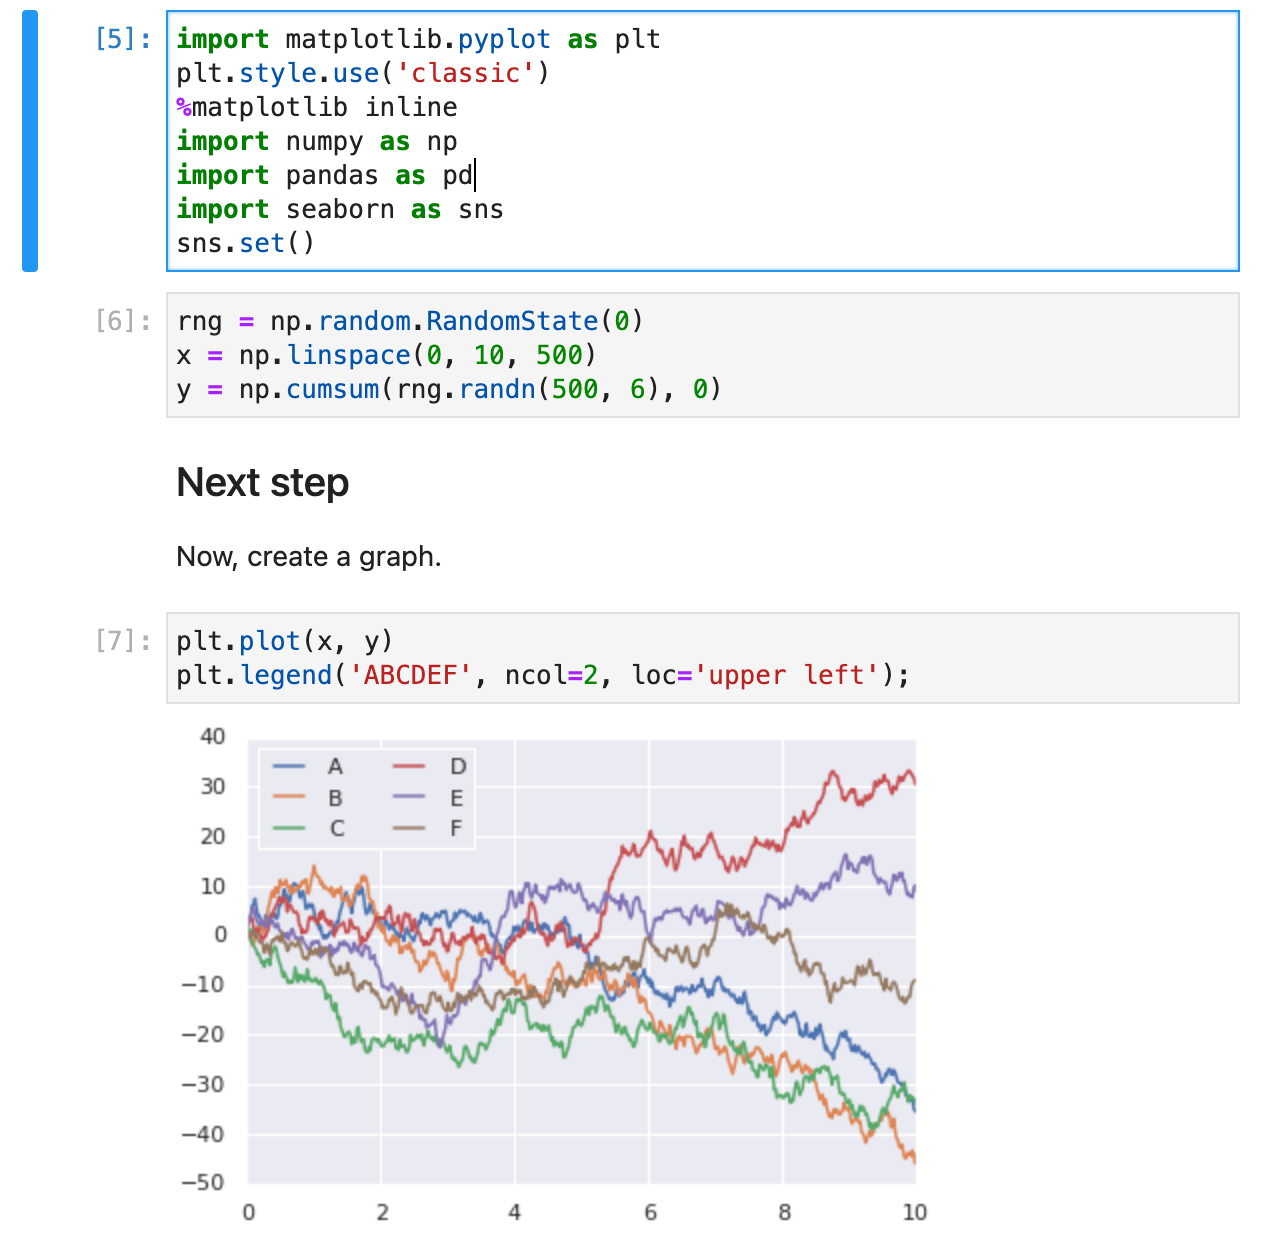
\includegraphics{img/jupyternotebook.png}

\subsection{Aside: What is a
notebook?}\label{aside-what-is-a-notebook-1}

\subsection{Aside: What is a
notebook?}\label{aside-what-is-a-notebook-2}

A notebook is a document that contains both \textbf{code} and
\textbf{narrative}:

\begin{itemize}
\tightlist
\item
  Rmarkdown (\texttt{.rmd})
  
\includegraphics[width=2.60417in,height=\textheight]{img/rlogo.png}
\end{itemize}

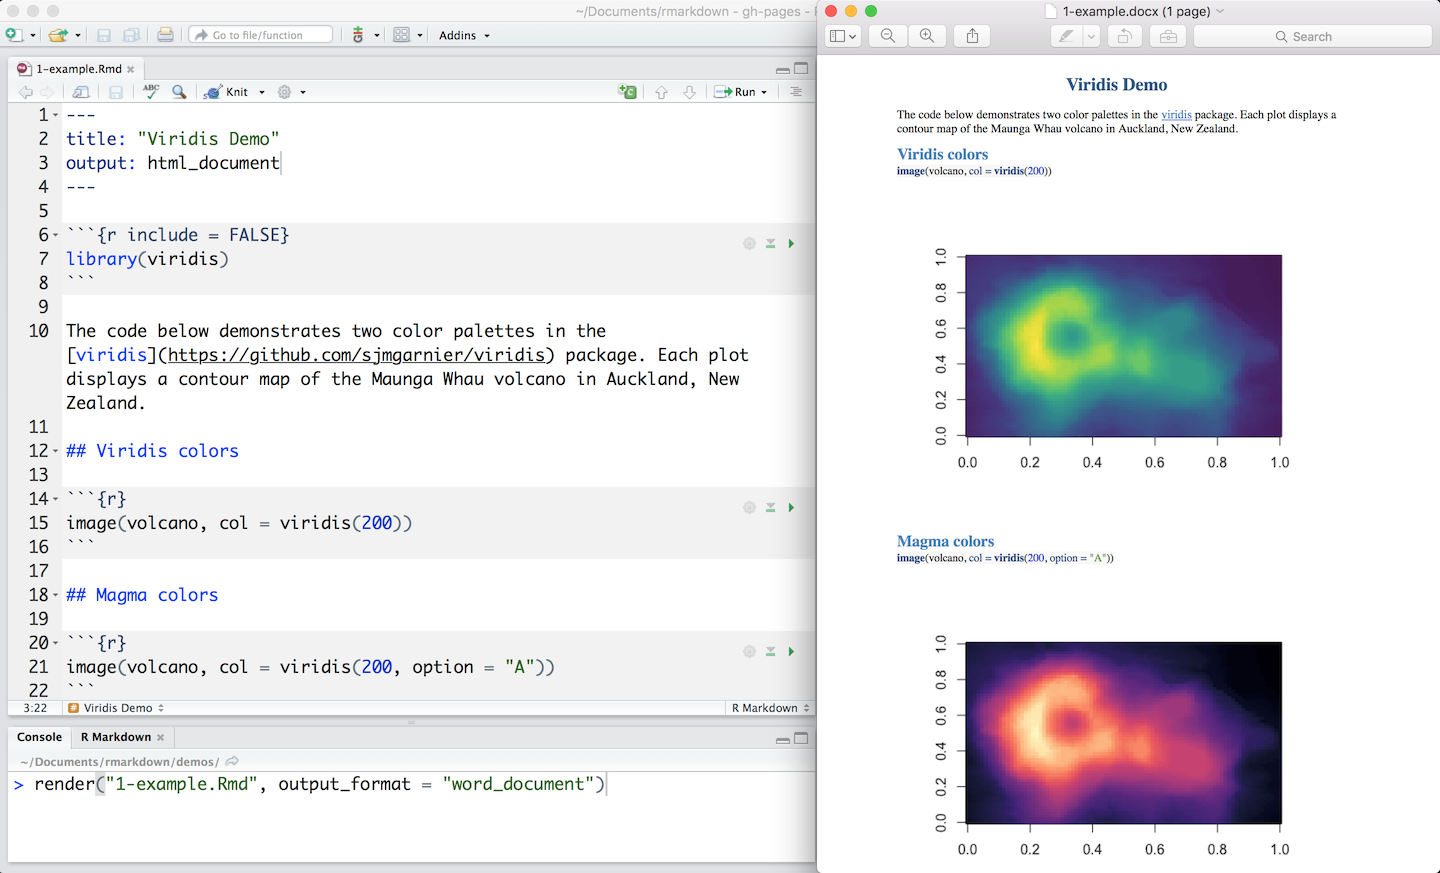
\includegraphics{img/rmarkdownexample.png}

\subsection{Aside: What is a
notebook?}\label{aside-what-is-a-notebook-3}

\subsection{Aside: What is a
notebook?}\label{aside-what-is-a-notebook-4}

A notebook is a document that contains both \textbf{code} and
\textbf{narrative}:

\begin{itemize}
\tightlist
\item
  Quarto document (\texttt{.qmd})
  
\includegraphics[width=3.64583in,height=\textheight]{img/quartologo.png}
\end{itemize}

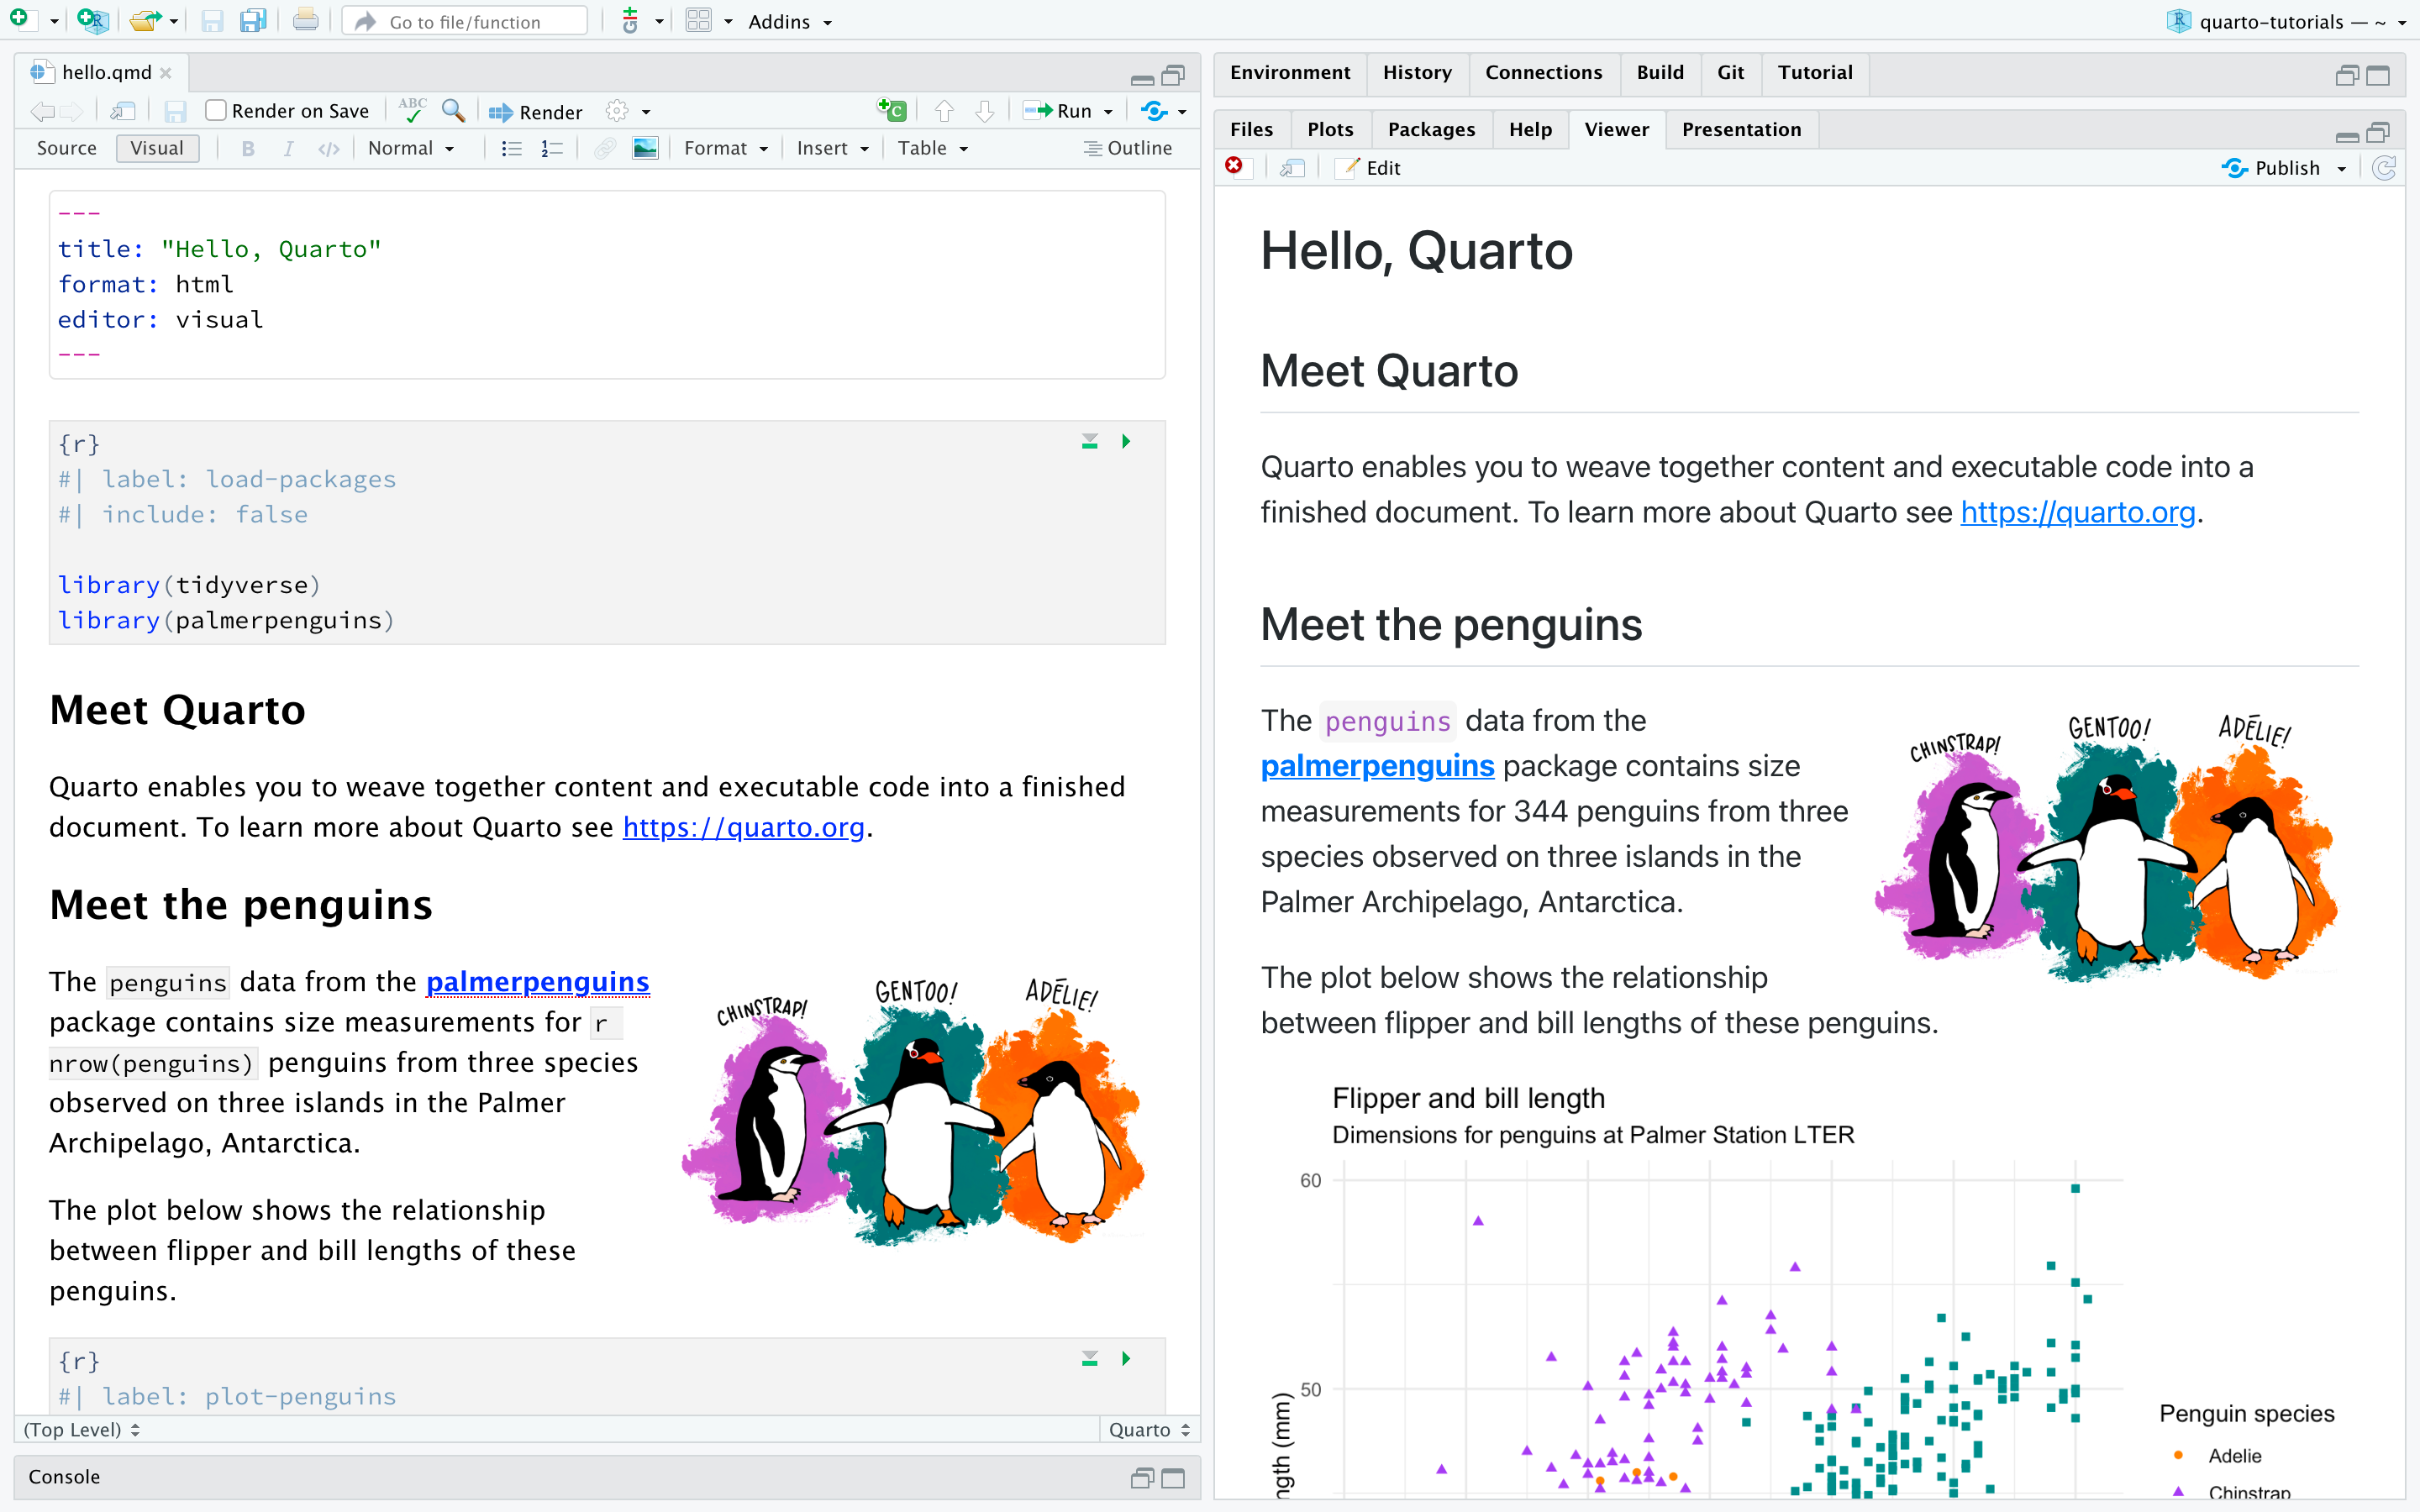
\includegraphics{img/quartopenguins.png}

\subsection{Aside: What are notebooks good
for?}\label{aside-what-are-notebooks-good-for}

\begin{itemize}
\item
  By combining narrative with code, researchers can share and explain
  what they did, how they did it, and why they did it.
\item
  Kind of like a research paper but with all the data, stats and
  computation baked in.
\item
  Great for teaching, communicating, and/or collaborating: where you can
  directly see what someone did, with helpful explanations along the
  way.
\end{itemize}

\subsection{Aside: Quick intro to R
Markdown}\label{aside-quick-intro-to-r-markdown}

Some markdown syntax

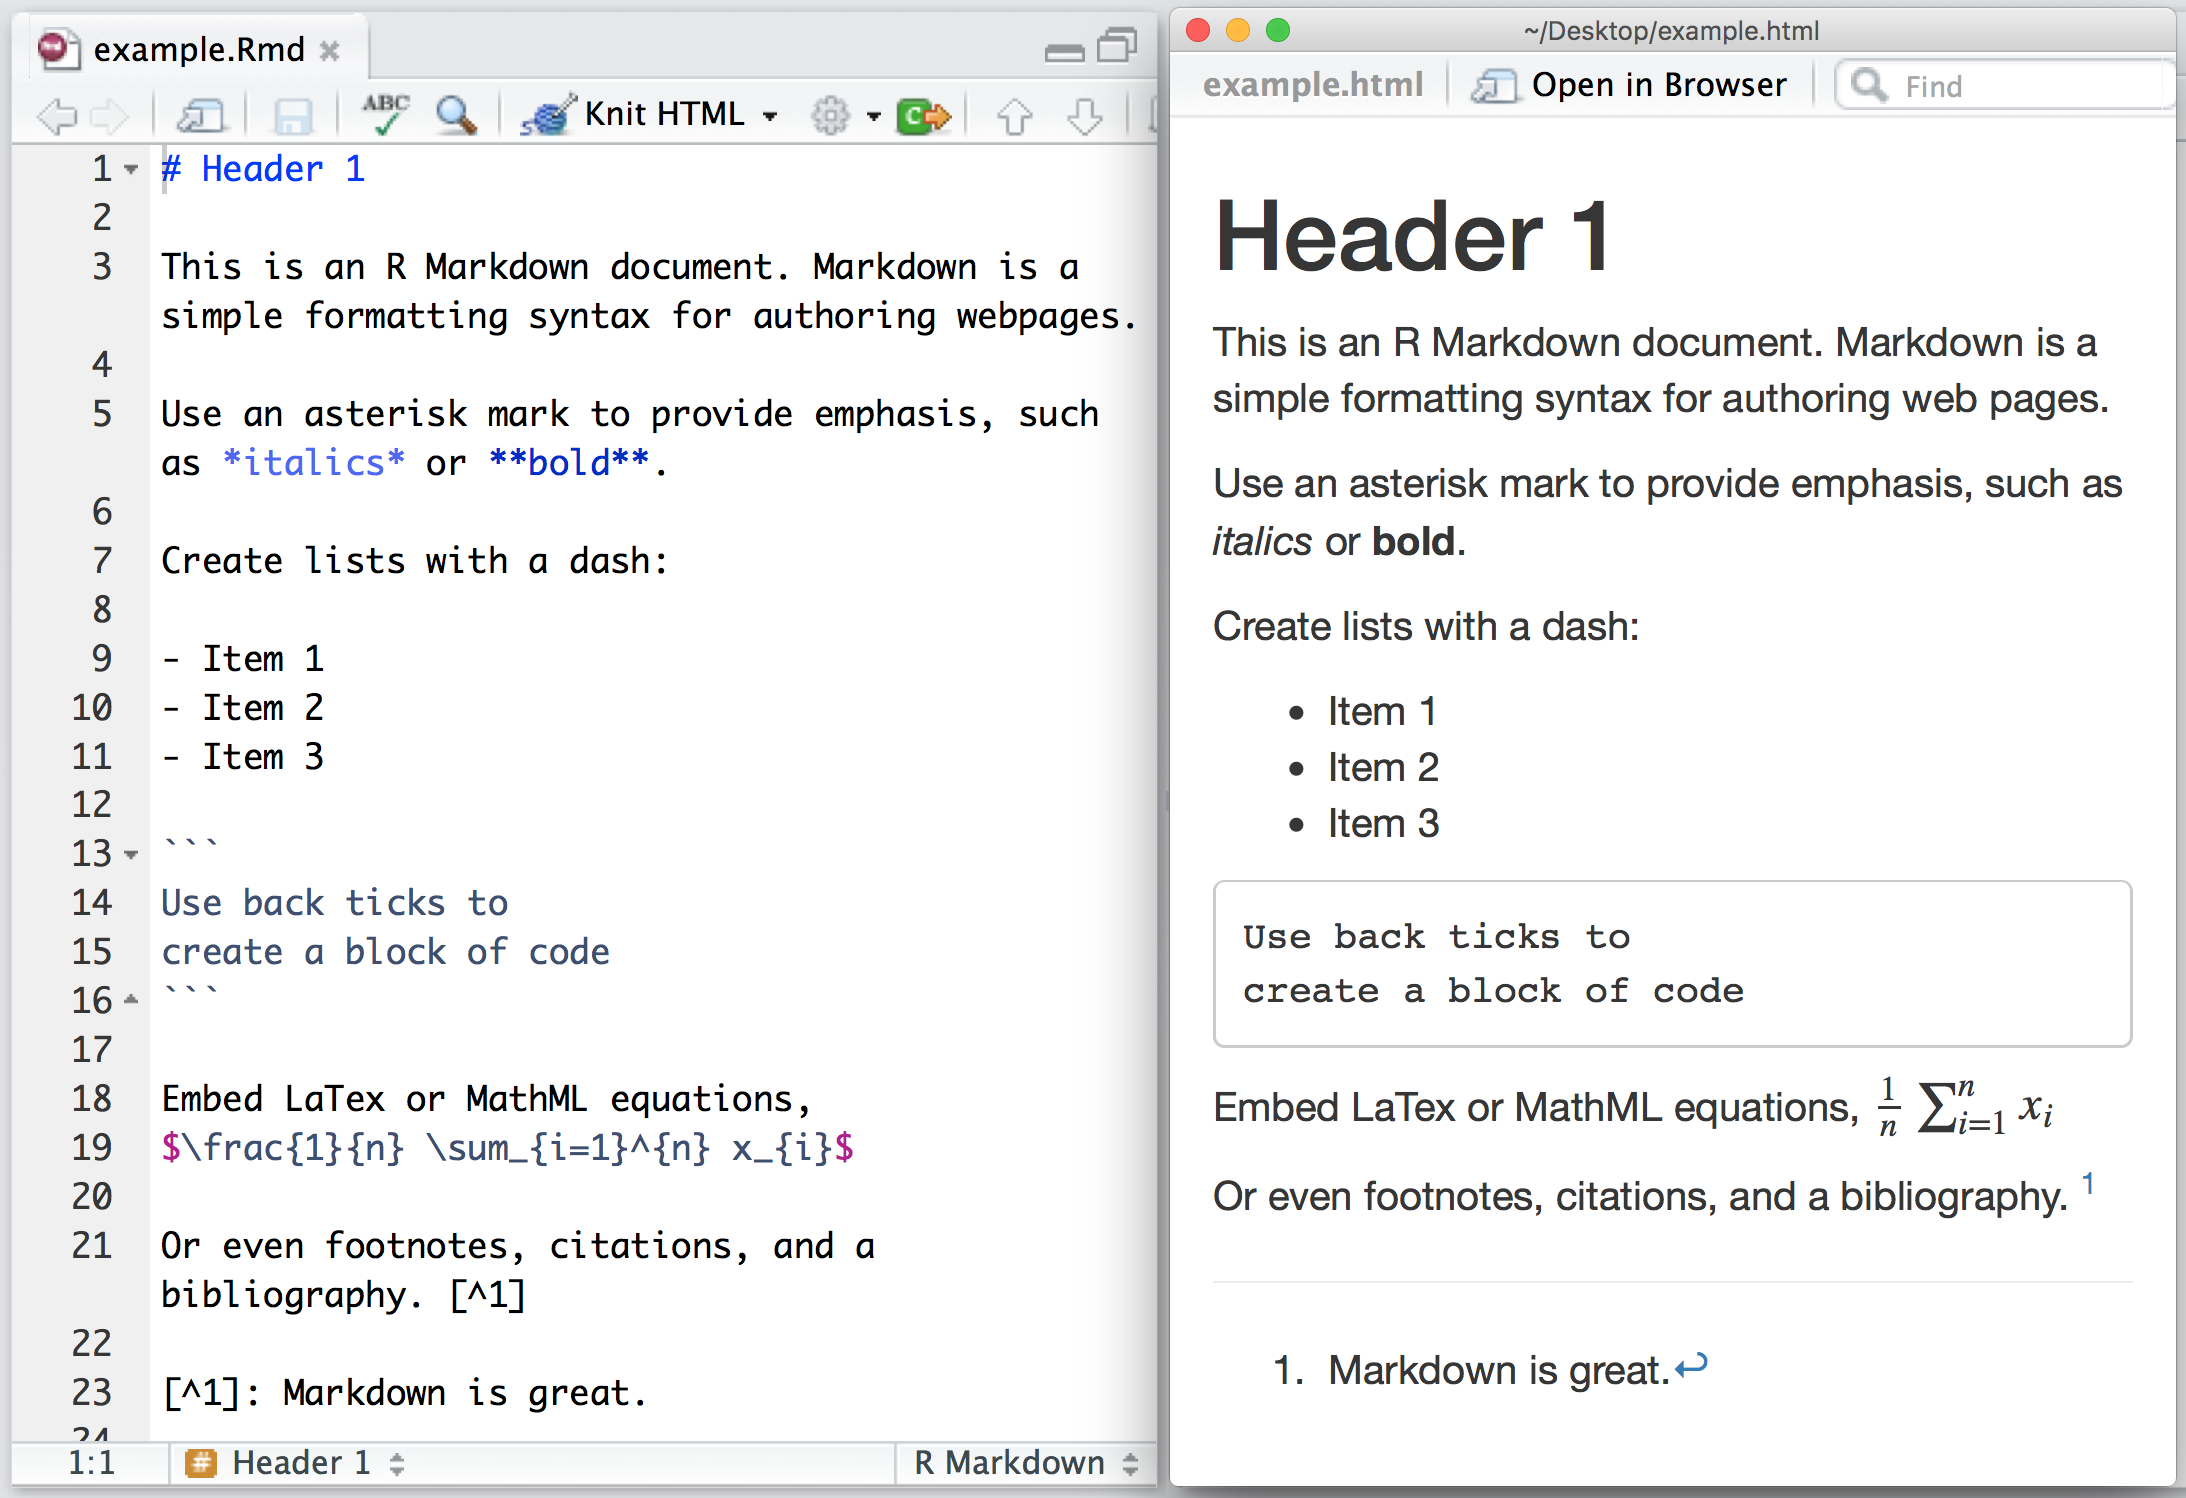
\includegraphics{img/markdown_ex.png}

\subsection{Aside: Quick intro to R
Markdown}\label{aside-quick-intro-to-r-markdown-1}

Markdown with evaluated code

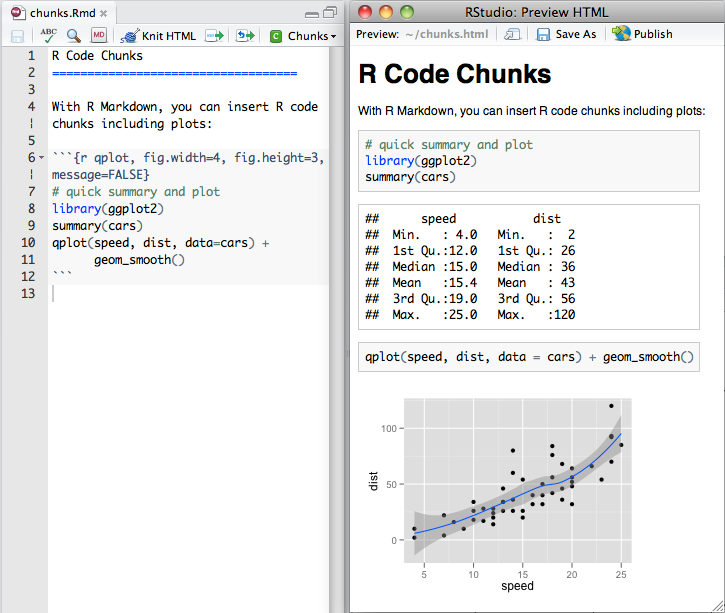
\includegraphics{img/rcode_ex.png}

\subsection{Aside: Quick intro to R
Markdown}\label{aside-quick-intro-to-r-markdown-2}

You can also include code inline (mixed in with the markdown text)

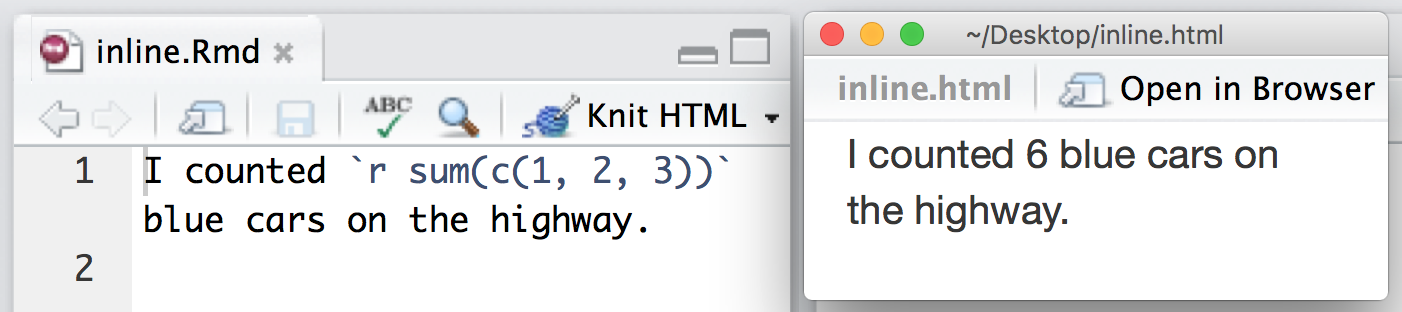
\includegraphics{img/inlinecode_ex.png}

\section{Overview of Quarto
Manuscript}\label{overview-of-quarto-manuscript}

\subsection{Project Files}\label{project-files}

\begin{itemize}
\tightlist
\item
  \texttt{index.qmd}: a notebook file where you write your article. This
  file contains:

  \begin{itemize}
  \tightlist
  \item
    document metadata, including article front matter (authors,
    affiliations, etc.) and Quarto options,
  \item
    the article body, written using special Quarto markdown syntax that
    allows you to add things like cross references and citations, and
  \item
    optionally, code, where you control if, or how, the code and its
    output appear in the article.
  \end{itemize}
\end{itemize}

\subsection{Project Files}\label{project-files-1}

\begin{itemize}
\tightlist
\item
  \texttt{\_quarto.yml}: a configuration file that identifies the
  project as a Quarto manuscript and controls how your manuscript is put
  together.
\end{itemize}

. . .

\begin{verbatim}
project:
  type: manuscript

execute:
  freeze: auto

format:
  html:
    toc: true
    comments:
      hypothesis: true
  docx: default
  jats: default
  nature-pdf:
    journal: "sn-nature"
    keep_tex: true
\end{verbatim}

\subsection{index.qmd}\label{index.qmd}

The file \texttt{index.qmd} is a Quarto markdown file. It contains three
types of content:

\begin{itemize}
\tightlist
\item
  Starts with a YAML header, used to set document metadata, including
  scholarly front matter. The YAML header starts and ends with a line of
  three dashes (\texttt{-\/-\/-})
\end{itemize}

\subsection{index.qmd}\label{index.qmd-1}

YAML header:

\begin{Shaded}
\begin{Highlighting}[]
\PreprocessorTok{{-}{-}{-}}
\FunctionTok{title}\KeywordTok{:}\AttributeTok{ La Palma Earthquakes}
\FunctionTok{author}\KeywordTok{:}
\AttributeTok{  }\KeywordTok{{-}}\AttributeTok{ }\FunctionTok{name}\KeywordTok{:}\AttributeTok{ Steve Purves}
\AttributeTok{    }\FunctionTok{orcid}\KeywordTok{:}\AttributeTok{ 0000{-}0002{-}0760{-}5497}
\AttributeTok{    }\FunctionTok{corresponding}\KeywordTok{:}\AttributeTok{ }\CharTok{true}
\AttributeTok{    }\FunctionTok{email}\KeywordTok{:}\AttributeTok{ steve@curvenote.com}
\AttributeTok{    }\FunctionTok{roles}\KeywordTok{:}
\AttributeTok{      }\KeywordTok{{-}}\AttributeTok{ Investigation}
\AttributeTok{      }\KeywordTok{{-}}\AttributeTok{ Project administration}
\AttributeTok{      }\KeywordTok{{-}}\AttributeTok{ Software}
\AttributeTok{      }\KeywordTok{{-}}\AttributeTok{ Visualization}
\AttributeTok{    }\FunctionTok{affiliations}\KeywordTok{:}
\AttributeTok{      }\KeywordTok{{-}}\AttributeTok{ Curvenote}
\AttributeTok{  }\KeywordTok{{-}}\AttributeTok{ }\FunctionTok{name}\KeywordTok{:}\AttributeTok{ Rowan Cockett}
\AttributeTok{    }\FunctionTok{orcid}\KeywordTok{:}\AttributeTok{ 0000{-}0002{-}7859{-}8394}
\AttributeTok{    }\FunctionTok{corresponding}\KeywordTok{:}\AttributeTok{ }\CharTok{false}
\AttributeTok{    }\FunctionTok{roles}\KeywordTok{:}\AttributeTok{ }\KeywordTok{[]}
\AttributeTok{    }\FunctionTok{affiliations}\KeywordTok{:}
\AttributeTok{      }\KeywordTok{{-}}\AttributeTok{ Curvenote}
\FunctionTok{license}\KeywordTok{:}\AttributeTok{ CC BY{-}SA 4.0}
\FunctionTok{keywords}\KeywordTok{:}
\AttributeTok{  }\KeywordTok{{-}}\AttributeTok{ La Palma}
\AttributeTok{  }\KeywordTok{{-}}\AttributeTok{ Earthquakes}
\FunctionTok{date}\KeywordTok{:}\AttributeTok{ }\StringTok{\textquotesingle{}2022{-}05{-}11\textquotesingle{}}
\FunctionTok{abstract}\KeywordTok{: }\CharTok{|}
\NormalTok{  In September 2021, a significant jump in seismic activity on the island of La Palma (Canary Islands, Spain) signaled the start of a volcanic crisis that still continues at the time of writing. Earthquake data is continually collected and published by the Instituto Geográphico Nacional (IGN). We have created an accessible dataset from this and completed preliminary data analysis which shows seismicity originating at two distinct depths, consistent with the model of a two reservoir system feeding the currently very active volcano.}
\FunctionTok{keypoints}\KeywordTok{:}
\AttributeTok{  }\KeywordTok{{-}}\AttributeTok{ You may specify 1 to 3 keypoints for this PDF template}
\AttributeTok{  }\KeywordTok{{-}}\AttributeTok{ These keypoints are complete sentences and less than or equal to 140 characters}
\AttributeTok{  }\KeywordTok{{-}}\AttributeTok{ }\StringTok{\textquotesingle{}They are specific to this PDF template, so they will not appear in other exports\textquotesingle{}}
\FunctionTok{citation}\KeywordTok{:}
\AttributeTok{  }\FunctionTok{container{-}title}\KeywordTok{:}\AttributeTok{ Notebooks Now!}
\FunctionTok{draft}\KeywordTok{:}\AttributeTok{ }\CharTok{false}
\FunctionTok{bibliography}\KeywordTok{:}\AttributeTok{ references.bib}
\FunctionTok{echo}\KeywordTok{:}\AttributeTok{ }\CharTok{false}
\PreprocessorTok{{-}{-}{-}}
\end{Highlighting}
\end{Shaded}

\subsection{index.qmd}\label{index.qmd-2}

\begin{itemize}
\item
  \texttt{index.qmd} body may include executable code chunks: start with
  three backticks followed by the code language in curly braces
  (e.g.~\texttt{\textasciigrave{}\textasciigrave{}\textasciigrave{}\{r\}}
  or
  \texttt{\textasciigrave{}\textasciigrave{}\textasciigrave{}\{python\}}).
\item
  The rest of the document interpreted as Quarto specific markdown,
  allowing you to include figures, tables, equations, cross references
  and citations.
\end{itemize}

\subsection{figures}\label{figures}

\texttt{!{[}An\ elephant{]}(/path/to/elephant.png)\{fig-elephant\}}

\begin{itemize}
\tightlist
\item
  Can be cross referenced with \texttt{@fig-elephant} in the document
\end{itemize}

. . .

\begin{figure}[H]

{\centering 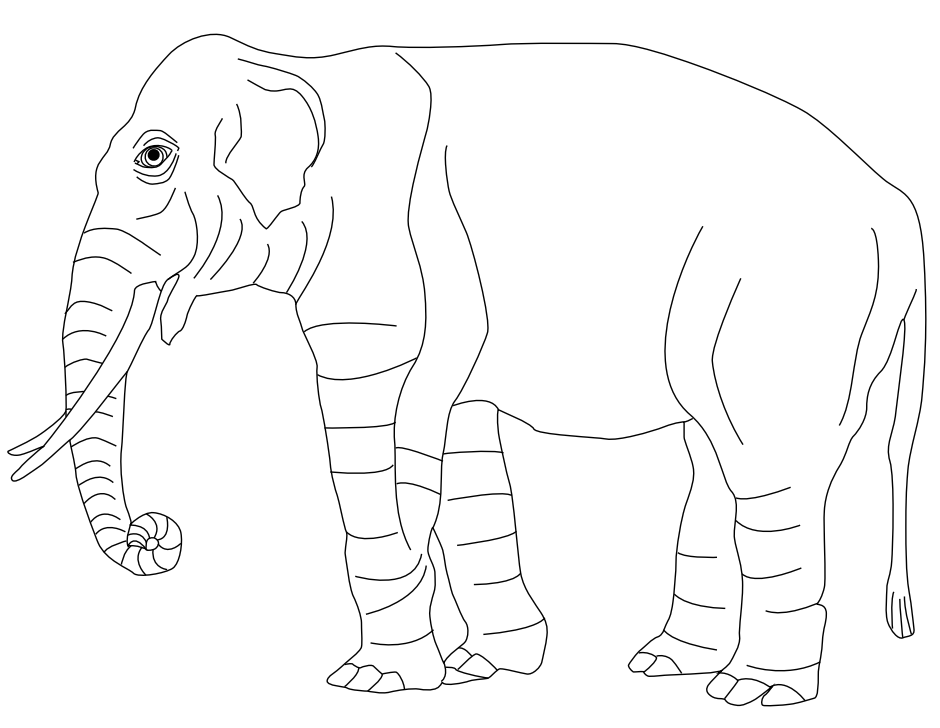
\includegraphics[width=4.16667in,height=\textheight]{img/elephant.png}

}

\caption{An elephant}

\end{figure}%

\subsection{figures}\label{figures-1}

\begin{itemize}
\tightlist
\item
  Can also be created using \texttt{R} or \texttt{Python}
\end{itemize}

. . .

\begin{verbatim}
```python
#| label: fig-plot
#| fig-cap: "Plot"
import matplotlib.pyplot as plt
plt.plot([1,23,2,4])
plt.show()
```
For example, see @fig-plot.
\end{verbatim}

\begin{center}
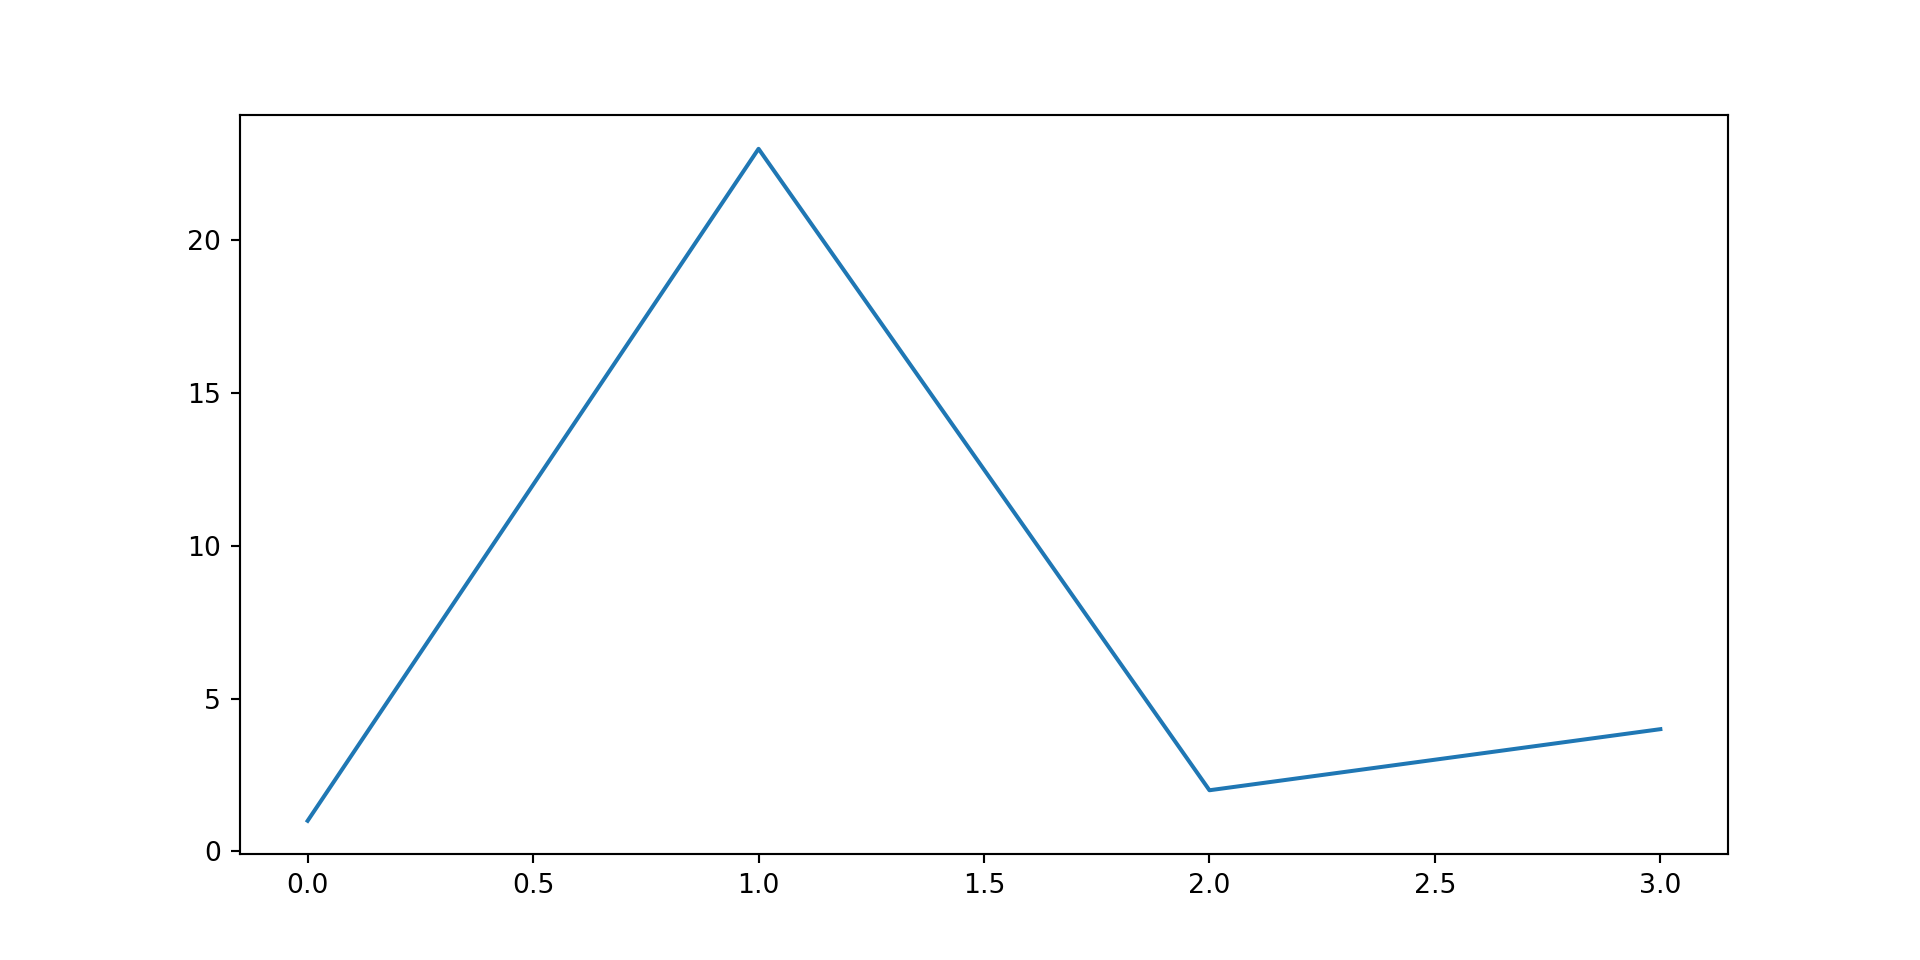
\includegraphics[width=6.25in,height=\textheight]{img/python.png}
\end{center}

\subsection{figures}\label{figures-2}

\begin{itemize}
\item
  Can also embed from a \texttt{.qmd} or \texttt{.ipynb} file:
  \texttt{\{\{\textless{}\ embed\ mycode.ipynb\#fig-plot\ \textgreater{}\}\}}
\item
  Which itself contains something like:
\end{itemize}

. . .

\begin{verbatim}
#| label: fig-plot
#| fig-cap: "Plot"
import matplotlib.pyplot as plt
plt.plot([1,23,2,4])
plt.show()
\end{verbatim}

\subsection{tables}\label{tables}

\begin{itemize}
\item
  This is probably the most complex element of Quarto
\item
  Easiest way is using markdown pipes (using RStudio Visual mode):
\end{itemize}

. . .

\begin{verbatim}
| Default | Left | Right | Center |
|---------|:-----|------:|:------:|
| 12      | 12   |    12 |   12   |
| 123     | 123  |   123 |  123   |
| 1       | 1    |     1 |   1    |

: Demonstration of pipe table syntax {#tbl-numbers}
\end{verbatim}

. . .

\begin{longtable}[]{@{}llrc@{}}
\toprule\noalign{}
Default & Left & Right & Center \\
\midrule\noalign{}
\endhead
\bottomrule\noalign{}
\endlastfoot
12 & 12 & 12 & 12 \\
123 & 123 & 123 & 123 \\
1 & 1 & 1 & 1 \\
\end{longtable}

\subsection{tables}\label{tables-1}

\begin{itemize}
\tightlist
\item
  You can also write your table in \texttt{R} or \texttt{Python}
\end{itemize}

. . .

\begin{verbatim}

#| label: tbl-planets
#| tbl-cap: Astronomical object

from IPython.display import Markdown
from tabulate import tabulate
table = [["Sun","696,000",1.989e30],
         ["Earth","6,371",5.972e24],
         ["Moon","1,737",7.34e22],
         ["Mars","3,390",6.39e23]]
Markdown(tabulate(
  table, 
  headers=["Astronomical object","R (km)", "mass (kg)"]
))
\end{verbatim}

. . .

\begin{center}
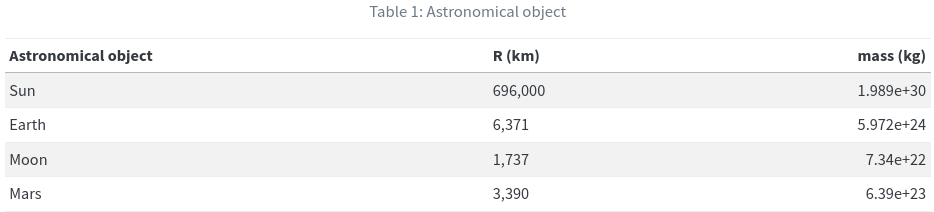
\includegraphics[width=8.33333in,height=\textheight]{img/table.png}
\end{center}

\subsection{tables}\label{tables-2}

\begin{itemize}
\tightlist
\item
  Can also write tables in \(\LaTeX{}\) (but may not be converted to
  HTML well, and vice versa)
\end{itemize}

. . .

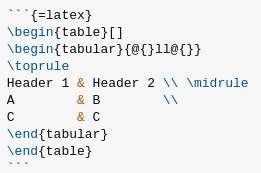
\includegraphics[width=2\textwidth,height=\textheight]{img/latextable.png}

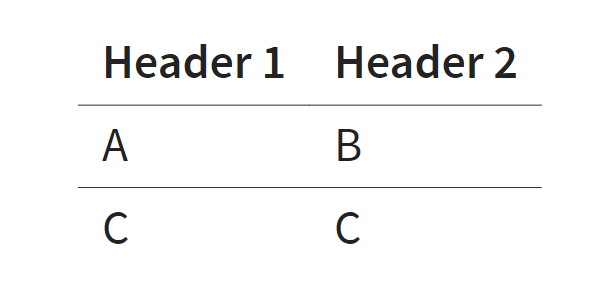
\includegraphics{img/latextablerendered.png}

\subsection{references}\label{references}

\begin{itemize}
\item
  References can be accomplished using a \texttt{.bib} file
\item
  Here is an example:
\end{itemize}

. . .

\begin{verbatim}
@article{ahmedDiamagneticComponentMap2023a,
  title = {The Diamagnetic Component Map from Quantitative Susceptibility Mapping ({{QSM}}) Source Separation Reveals Pathological Alteration in {{Alzheimer}}'s Disease-Driven Neurodegeneration},
  author = {Ahmed, Maruf and Chen, Jingjia and Arani, Arvin and Senjem, Matthew L. and Cogswell, Petrice M. and Jack, Clifford R. and Liu, Chunlei},
  year = {2023},
  month = oct,
  journal = {NeuroImage},
  volume = {280},
  pages = {120357},
  issn = {1095-9572},
  doi = {10.1016/j.neuroimage.2023.120357},
  langid = {english},
  pmid = {37661080},
  keywords = {Alzheimer Disease,Alzheimer's disease,Brain,Cerebral Cortex,DECOMPOSE,Demyelination,Disease Progression,Gray Matter,Humans,Magnetic susceptibility,Neurodegeneration,Quantitative susceptibility mapping}
}
\end{verbatim}

\begin{itemize}
\tightlist
\item
  referenced in the document with
  \texttt{@ahmedDiamagneticComponentMap2023a}
\end{itemize}

\subsection{in-line code}\label{in-line-code}

\begin{itemize}
\item
  You can also mix text with in-line code, in order to reference
  variables
\item
  For example:
\end{itemize}

. . .

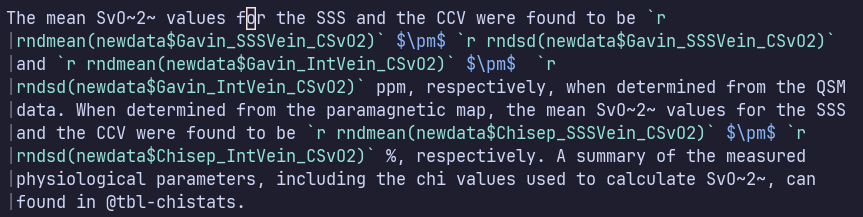
\includegraphics{img/inlinecode.png}

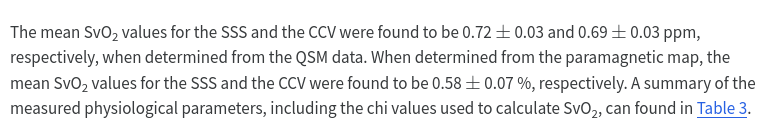
\includegraphics{img/inlinecode_rendered.png}

\section{Simple Demonstration with
Quarto}\label{simple-demonstration-with-quarto}

\subsection{Let's write a manuscript}\label{lets-write-a-manuscript}

\begin{itemize}
\item
  First, install quarto
  \url{https://quarto.org/docs/download/prerelease.html}
\item
  Approach 1: Start from scratch

  \begin{itemize}
  \tightlist
  \item
    Creating a Quarto manuscript

    \begin{itemize}
    \tightlist
    \item
      RStudio: New Project \textgreater{} New Directory \textgreater{}
      Quarto Manuscript
    \item
      \texttt{quarto\ create\ project\ manuscript\ \textless{}name\textgreater{}}
    \end{itemize}
  \item
    Add manuscript content
  \end{itemize}
\item
  Approach 2: Start with a sample from
  \url{https://quarto.org/docs/manuscripts}
\end{itemize}

\subsection{Let's write a manuscript}\label{lets-write-a-manuscript-1}

\begin{itemize}
\item
  We will then need to decide what tool we will use:
  
\includegraphics{img/editors.png}
\item
  Today I will use RStudio as an example
\end{itemize}

\subsection{Let's write a manuscript}\label{lets-write-a-manuscript-2}

\begin{itemize}
\tightlist
\item
  Clone the Template Repository

  \begin{itemize}
  \tightlist
  \item
    Head to
    \url{https://github.com/quarto-ext/manuscript-template-rstudio/generate}
    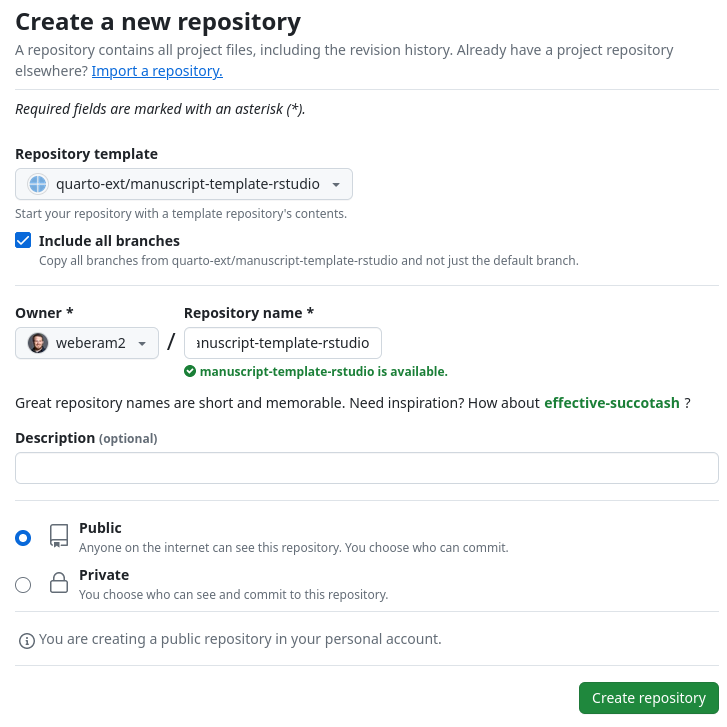
\includegraphics{img/github_repo.png}
  \end{itemize}
\end{itemize}

\subsection{Let's write a manuscript}\label{lets-write-a-manuscript-3}

\begin{itemize}
\tightlist
\item
  Once your repository is created, clone it to your local computer.
\item
  In RStudio, you can do: \textbf{File} \textgreater{} \textbf{New
  Project}.
\item
  In the \textbf{New Project} dialog, select \textbf{From Version
  Control}, then \textbf{Git}, and copy and paste the repo URL from
  GitHub. 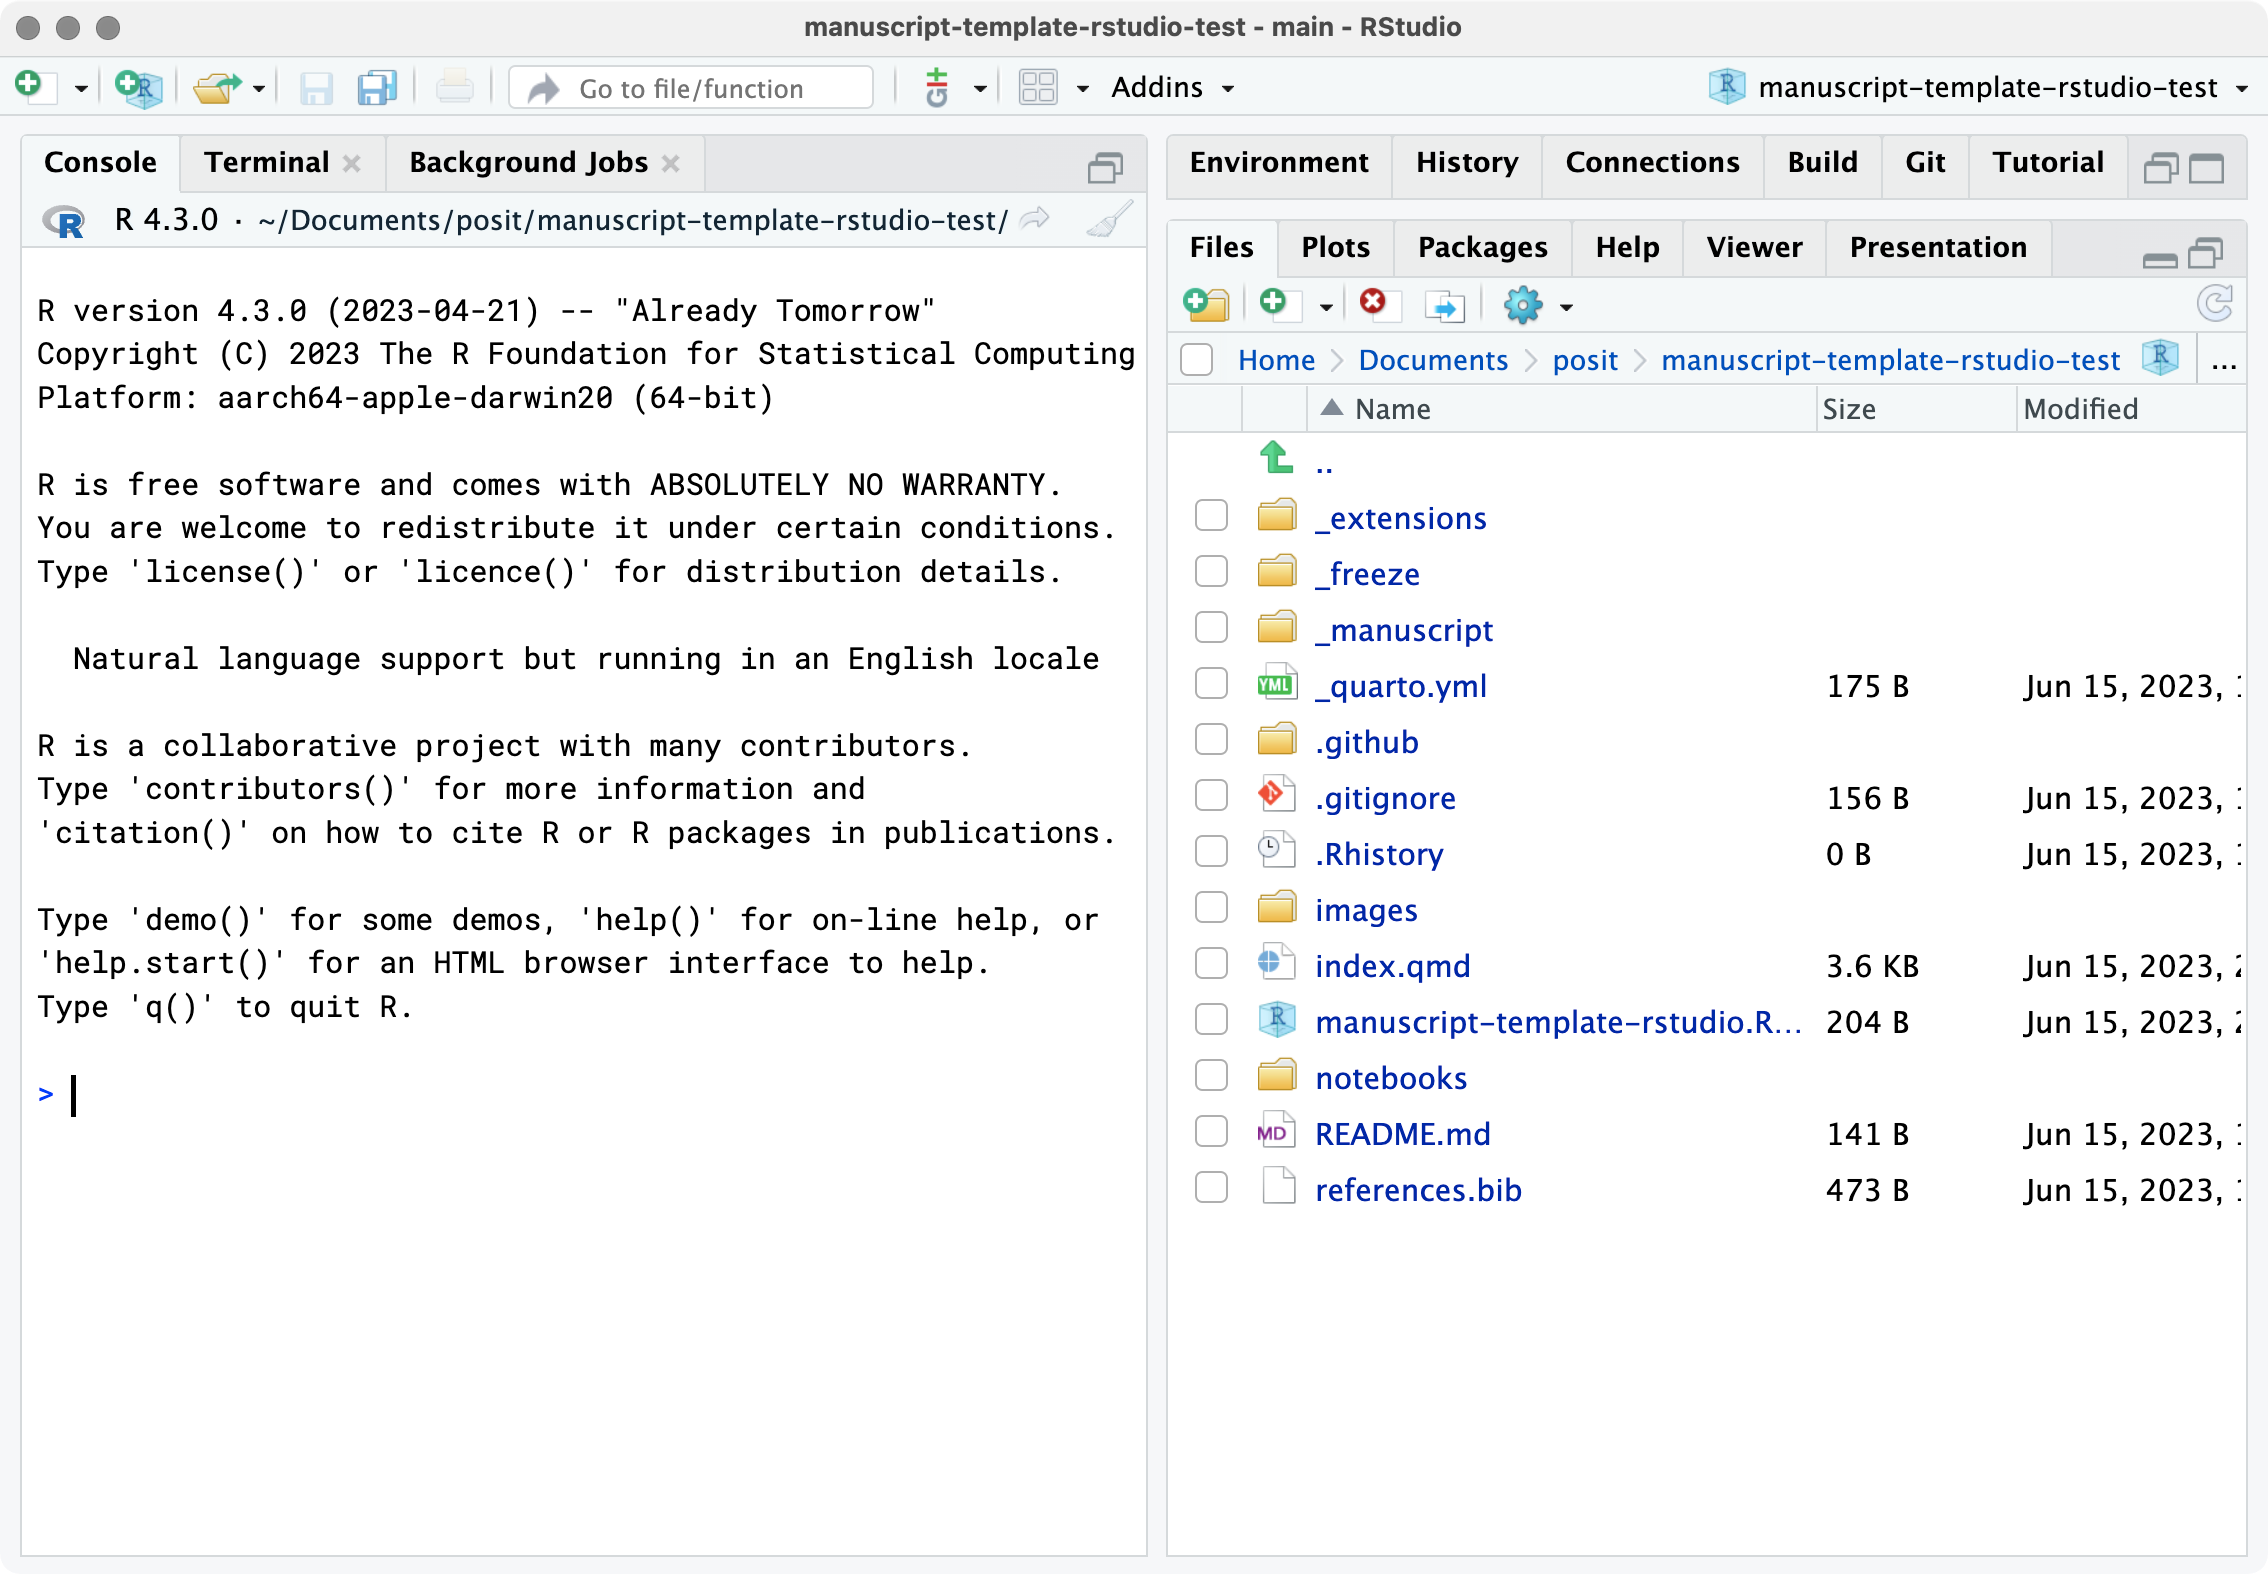
\includegraphics{img/rstudio_git_manuscript.png}
\end{itemize}

\subsection{Workflow}\label{workflow}

\begin{itemize}
\item
  The basic workflow for writing a manuscript in Quarto is to make
  changes to your article content in \texttt{index.qmd}, preview the
  changes with Quarto, and repeat.
\item
  Render and preview the manuscript by hitting the \textbf{Render}
  button located in the menu bar of the editor (RStudio in this case):
  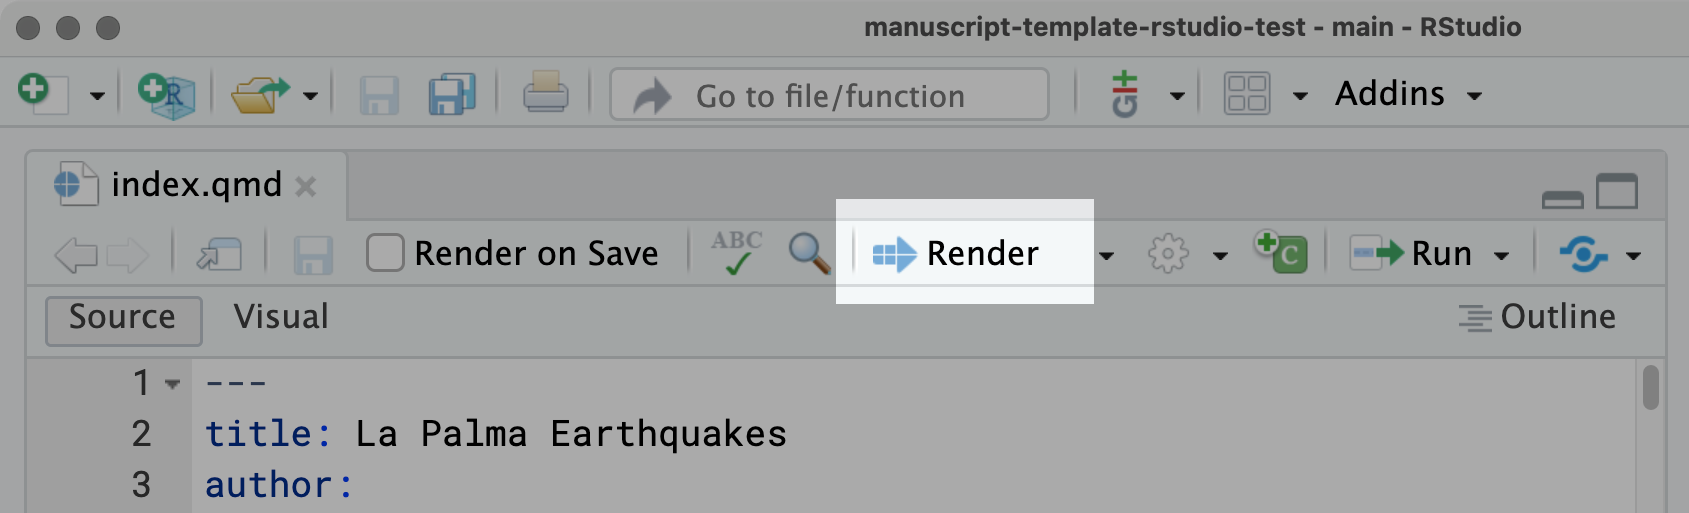
\includegraphics{img/renderbutton.png}
\end{itemize}

\subsection{Let's write a manuscript}\label{lets-write-a-manuscript-4}

You'll see some output from Quarto in the Background Jobs pane and then
a live preview will appear in the Viewer pane.

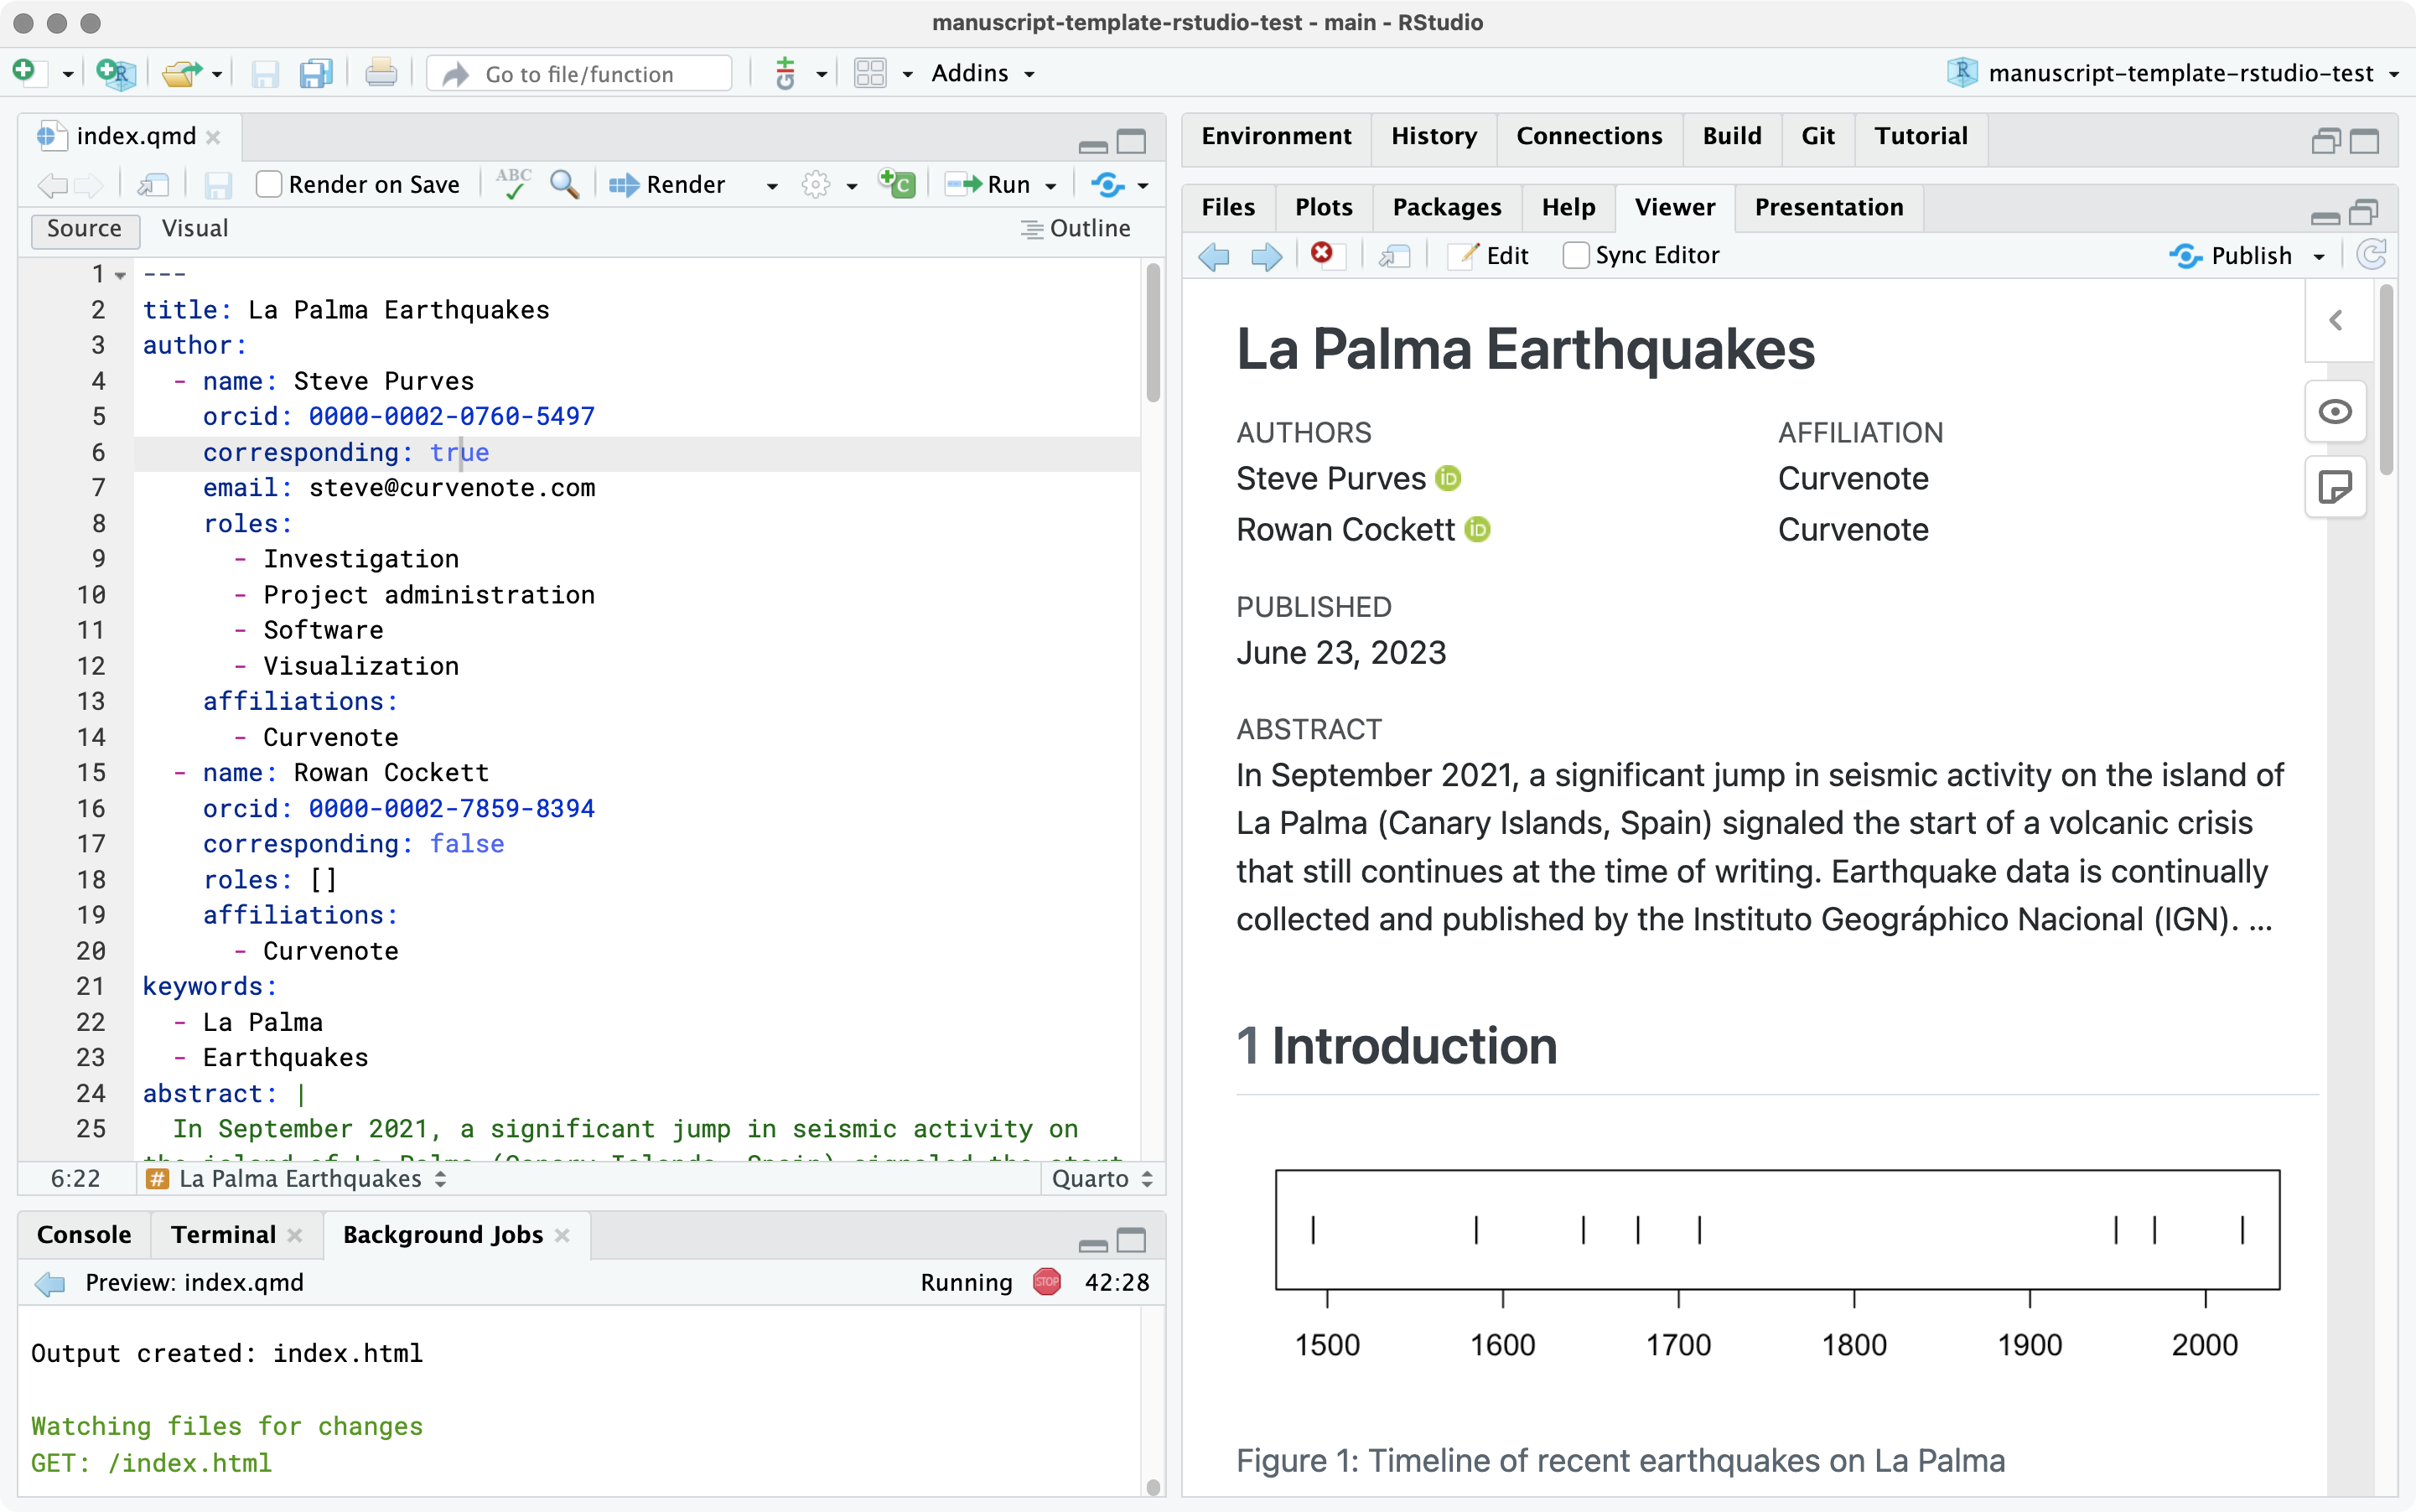
\includegraphics{img/quartopreview.png}

\subsection{Let's write a manuscript}\label{lets-write-a-manuscript-5}

What does \textbf{Render} do?


\includegraphics{img/quarto_howitworks.png}

\begin{itemize}
\item
  \textbf{knitr} executes the code chunks and creates a new markdown
  (\texttt{.md}) document, which includes the code and its output
\item
  the \texttt{.md} file is then processed by \textbf{pandoc}, which
  translates markdown/HTML/\(\LaTeX{}\) into various output formats
\end{itemize}

\subsection{Let's write a manuscript}\label{lets-write-a-manuscript-6}

Open RStudio

\section{Real life demonstration}\label{real-life-demonstration}

\subsection{Open Neovim}\label{open-neovim}

\section{What's Next?}\label{whats-next}

\subsection{Collaborating}\label{collaborating}

\begin{itemize}
\item
  Most people will be happy to use the \texttt{.docx} and track changes
\item
  Others may wish to publish their page on Github and use the annotation
  tool 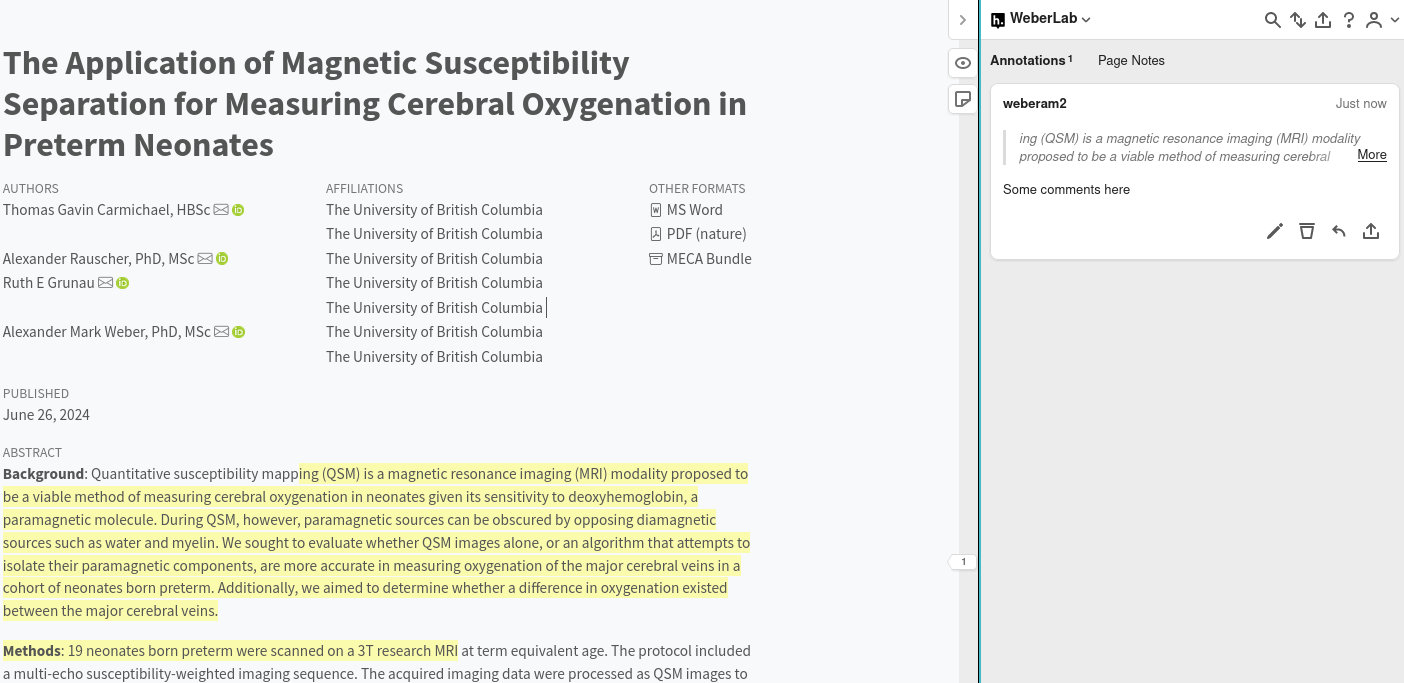
\includegraphics{img/annotate.png}
\end{itemize}

\subsection{Collaborating}\label{collaborating-1}

\begin{itemize}
\tightlist
\item
  Brave souls may wish to make changes to the \texttt{.tex} file and
  track changes with \texttt{latexdiff}
  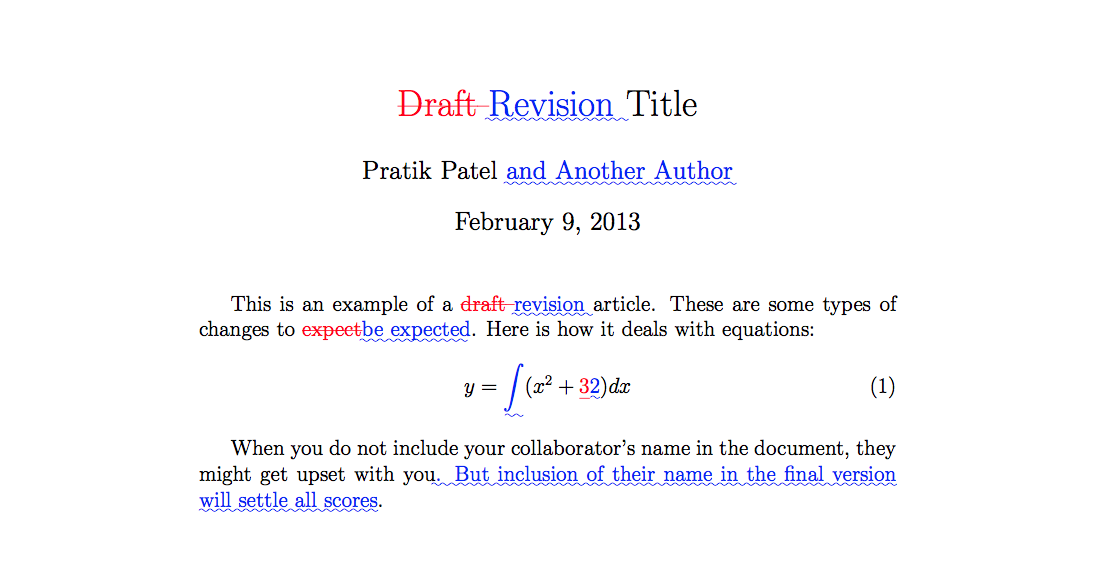
\includegraphics{img/latexdiff.png}
\end{itemize}

\subsection{Publishing}\label{publishing}

\begin{itemize}
\item
  Journal will usually want the file in \texttt{.docx}, sometimes they
  accept \texttt{.tex}, and rarely they will take \texttt{.pdf} for
  reviewing and then require the \texttt{.docx} or \texttt{.tex} file
  once accepted
\item
  But \texttt{.pdf}s are static\ldots{} how will people be able to see
  your source code once your paper is published?
\item
  Publish your HTML manuscript on Github (or other alternatives) and
  cite your page in your pdf, perhaps in the \textbf{Data Availability}
  section
\item
  Can add a \textbf{binder} using \texttt{quarto\ use\ binder} and
  including \texttt{code-links:\ binder} in your \texttt{\_quarto.yml}
  file
\end{itemize}

\subsection{Publishing}\label{publishing-1}

\begin{itemize}
\item
  \href{https://neurolibre.org/}{Neurolibre}
\item
  \href{https://data.agu.org/notebooks-now/}{Notebooks Now!}
\item
  \href{https://elifesciences.org/articles/52258/executable}{eLife
  example}
\end{itemize}

\section{Criticisms}\label{criticisms}

\subsection{What are some barriers?}\label{what-are-some-barriers}

\begin{itemize}
\tightlist
\item
  Conversion to different outputs is not always straightforward, and
  sometimes may not be possible to replicate what you want
\item
  Getting complex tables to work in HTML and \(\LaTeX{}\)
\item
  Steep learning curve
\item
  No career incentive to try this new approach (i.e.~``who has the
  time?'')
\item
  Slow to preview/render
\item
  Errors/bugs can be frustrating (this is where a good text editor can
  be incredibly handy)
\end{itemize}

\subsection{What are some criticisms?}\label{what-are-some-criticisms}

\begin{itemize}
\tightlist
\item
  ``But people will take my analysis, run it another way, and say my
  results aren't valid''
\item
  ``This looks hard, I don't want to have to learn \emph{another} new
  thing''
\end{itemize}

\subsection{What are some criticisms?}\label{what-are-some-criticisms-1}

\section{Summary}\label{summary}

\subsection{Summary}\label{summary-1}

In this talk, we learned about

\begin{itemize}
\tightlist
\item
  What a reproducible manuscript is,
\item
  Some reasons why scientists should be writing their manuscripts this
  way,
\item
  What Markdown, Knitr, Pandoc, LaTeX, Jupyter Notebook, R/RMarkdown,
  and Quarto are,
\item
  The basics of the syntax for Markdown, R and Quarto,
\item
  How to integrate author information, code, equations, tables, images,
  and citations
\item
  How to start writing your next manuscript using Quarto Manuscripts
\end{itemize}

\subsection{Resources}\label{resources}

\begin{itemize}
\item
  \faIcon{link} \url{https://quarto.org/docs/get-started/}
\item
  \faIcon{link} \url{https://quarto.org/docs/guide/}
\item
  \faIcon{link} \url{https://quarto.org/docs/manuscripts}
\item
  \faIcon{link} \url{https://www.learnlatex.org/en/}
\item
  \faIcon{link} \url{https://www.markdownguide.org/}
\end{itemize}

\subsection{Resources}\label{resources-1}

\begin{itemize}
\tightlist
\item
  \faIcon{book}
  \url{https://press.princeton.edu/books/hardcover/9780691222738/data-science-for-neuroimaging}
  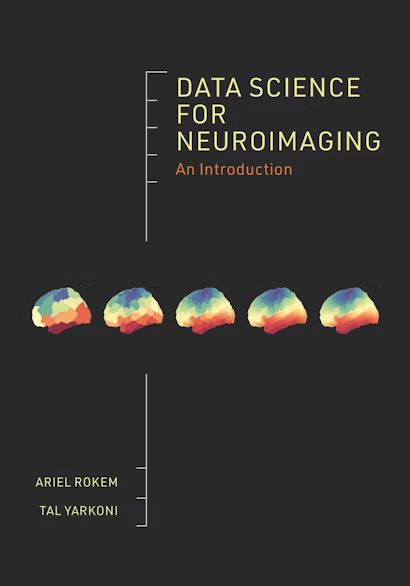
\includegraphics{img/datascienceneuroimag.png}
\end{itemize}

\subsection{Thank you}\label{thank-you}

\faIcon{github}
\url{https://github.com/weberam2/ReproducibleManuscriptTalk}

\faIcon{envelope}
\href{mailto:aweber@bcchr.ca}{\nolinkurl{aweber@bcchr.ca}}



\end{document}
